\documentclass[12pt]{article}
\usepackage{soul}
\usepackage{parskip}
\usepackage{amsfonts, amsmath, amssymb}
\usepackage{dcolumn, multirow}
\usepackage{setspace}
\usepackage{epsfig, subcaption, subfloat, graphicx}
\usepackage{tabularx}
\usepackage{anysize, indentfirst, setspace}
\usepackage{verbatim, rotating}
\usepackage{latexsym}
\usepackage{amsthm}
\usepackage{fullpage}
\usepackage{longtable}
\usepackage{natbib}
\usepackage{graphicx}
\usepackage{mathabx}
\usepackage{txfonts}
\usepackage{amsfonts}
\usepackage{stmaryrd}
\usepackage{mathrsfs}
\usepackage{dsfont}
\usepackage{comment}
\usepackage{url}
\usepackage{rotating}
\usepackage{appendix}
\usepackage[right=1in, left=1in, top=1in, bottom=1in]{geometry}
\usepackage{pdflscape}
\usepackage{float}
\usepackage{etoolbox}
\usepackage{hyperref}
\usepackage{booktabs}
\usepackage{lscape}
\usepackage{color}
%\BeforeBeginEnvironment{tabular}{\footnotesize}


\floatplacement{table}{!htbp}

\title{Viral Voting: Social Networks and Political Participation}
\date{\today}

\author{Nicholas Eubank,\footnote{Center for the Study of Democratic Institutions, Vanderbilt University, \href{mailto:nick@nickeubank.com}{nick@nickeubank.com}} \\ Guy Grossman,\footnote{Department of Political Science, University of Pennsylvania and \href{http://egap.org/}{EGAP}, \href{mailto:ggros@sas.upenn.edu}{ggros@sas.upenn.edu}} \\ Melina Platas,\footnote{Department of Political Science, New York University Abu Dhabi, \href{mailto:mplatas@nyu.edu}{mplatas@nyu.edu}} \\ Jonathan Rodden\footnote{Department of Political Science, Stanford University, \href{mailto:jrodden@stanford.edu}{jrodden@stanford.edu}}}

\providecommand{\keywords}[1]{\textbf{Key words:} #1}
% This is the beginning of a real document!
\begin{document}
\maketitle

\iffalse
\begin{center}
\textbf{Word Count}\\
Abstract: 165\\
Body: 5,288\\
Bibliography: 592\\
Total: 5,880
\end{center}
\fi


\begin{abstract}
    \noindent Social context theory suggests that an important driver of political participation is the behavior of family, friends, co-workers and neighbors. How do social ties between individuals shape equilibrium behavior in larger populations?  Despite theoretical inroads into this question, direct empirical tests remain scarce due to data limitations. We fill this gap using full social network data from 15 villages in rural Uganda, where village-level turnout is the outcome of interest.  We find that levels of participation predicted by structural features of village networks are strongly associated with actual village-level turnout in low-salience local elections, and weakly associated in high-salience presidential elections. We also find that these features predict other forms of political participation, including  attending village meetings and contributing to village projects. In addition to demonstrating that networks help explain political participation, we provide evidence that the mechanism of influence is that proposed by social context theory rather than alternative mechanisms like the presence of central brokers or the ability of networks to diffuse information.
\end{abstract}

\keywords{Turnout, networks, social context, Africa}

\pagebreak
\doublespace

When do voting and other forms of political participation go viral? Individuals' voting behavior can often be traced to that of their peers, and voting behavior is sensitive to social pressure~\citep{ioannides2013neighborhoods,Gerber:2008fs}. When does voting spread across entire social networks, resulting in high voter turnout, and when does it die out? While our social ties define who is likely to directly influence our behavior, scholars have suggested that it is the \emph{structure} of whole networks that determines how changes in individuals' behavior interact to shape equilibrium behavior in broader populations \citep{Siegel:2009vi,Sinclair:2012tq,Rolfe:2012ka,Fowler:2005ts,Larson:2016vk}.

Social context theory posits that an individual's likelihood of political participation is determined by two components: a personal disposition to participate and the level of participation among one's peers \citep{Fowler:2005ts,Siegel:2009vi,Rolfe:2012ka}. The distribution of personal dispositions, the network location of those with a high disposition toward participation, and the structure of the network as a whole, all affect whether a few social entrepreneurs can generate high levels of participation within the network.  Due to data constraints, however, the implications of this theory are rarely tested in real-world (as compared to fully simulated) settings.

In this paper we use complete network data from 15 rural villages in Uganda to examine whether structural features of social networks can explain when voting goes viral.  We find that they can.  Predicted levels of participation based on network properties are associated with real-life voter turnout within the network. This relationship holds strongly for low-salience local elections, and weakly for high-salience presidential elections. This latter finding suggests that peer influence and structural features of social networks will not always matter equally for voter turnout. Rather, features of social networks are likely to matter most in low salience elections where many voters may lack motivation to vote in the absence of prompting from politically inclined peers. We find suggestive evidence that is consistent with the idea that the role social networks are playing is in supporting social norms about voting~\citep{rosenzweig2019social} rather than coordinating voting behavior around a particular candidate. Like earlier work by~\citet{Gerber:2008fs}, this suggests a role for extrinsic motivations for voting, especially in low salience elections where intrinsic motivations may be weaker or voters may have weaker preferences over candidates.

Specifically, we build on simulation methods from \cite{Siegel:2009vi} and \cite{Rolfe:2012ka} to estimate the Theoretically-predicted level of Political Participation (TPP) that these networks should generate if social context theory is correct. We then test whether these predicted levels of participation correspond with actual voter turnout, %and village meeting attendance,
and consistent with social context theory, we find they are strongly positively correlated. We then present a set of analyses designed to go beyond the observation that ``networks matter,'' and explicitly test whether the specific mechanism of network influence that social context theorists describe are indeed at work.

First, we draw upon the rich data collected alongside our network data to validate our results. We show that villages with high TPP also have substantially higher attendance at village meetings, and have somewhat higher contributions to village projects (in time, cash, or labor), providing two more data points in support of social context theory. Using lab-in-the-field behavioral games, we rule out the possibility that network structure and political participation are both being driven by individual-level other-regarding preferences. And consistent with social context theory, we find that social networks appear to be substantially more important in the lower-salience elections for district chairperson, where news media is unlikely to provide information on the behavior of others, than in the high-salience presidential election, where information about the participation decisions of fellow citizens comes not only from peer-to-peer networks but also from news, rallies, and the like.

Second, we test whether our results may be driven by other mechanisms than those suggested by social context theory. We do so by measuring various features of network structure that would shape political participation if network influence was operating through a channel other than that proposed by social context theory. For example, one common theory for network influence is that networks \emph{diffuse information} that drive participation, by either increasing awareness of elections and candidates~\citep{mcclurg2003social}, or by applying social pressure~\citep{EubankKronick, larson2017west}. As we show, however, information diffusion simulations generate different predictions about which networks should support high political participation than do social context models, and our social context measures continue to predict turnout even when controlling for the efficiency with which a network spreads information. Similarly, theories of brokers suggest that network influence works through the presence of high-centrality individuals~\citep{Rojo:2014vw}. However, we show that our social-context-derived measure is not just proxying for the presence of high-centrality individuals by re-running our estimates without the highest degree nodes, a subsetting which only strengthens our results.

Through these exercises, we are able to provide novel, consistent evidence in support of the idea that the \emph{mechanism} of network influence is that described by social context theory.

\section{Social Context Theory}


Our analysis focuses on the ``social context'' model of social influence, which posits that an individual's likelihood of political participation is determined by two components: a personal disposition to participate, perhaps correlated with factors such as income, gender and education~\citep{wolfinger1980votes}, and the level of participation among one's peers \citep{Fowler:2005ts,Siegel:2009vi,Rolfe:2012ka}. According to this model, while some people will always be inclined to participate politically---individuals labeled ``unconditional'' decision makers by~\citet{Rolfe:2012ka} and ``rabble-rousers'' by~\citet{Siegel:2009vi}---others will only participate if they observe sufficient levels of participation among their peers.

The influence of social context has been documented in psychology experiments~\citep{ross2011person}.  In some cases, mirroring behavior may be the result of Bayesian updating by rational agents about the desirability of a behavior or strategic social conformity~\citep{goyal2012connections}, but research also suggests this dynamic may not be fully conscious~\citep{Cialdini:2015gt}.

While this mechanism of influence has been well-documented among individuals, the dynamics of diffusion to larger populations has received less empirical attention. This is due to the fact that social context models assume fundamental interdependencies in behavior that require the use of complete network analysis for studying macro social influence processes. If we wish to understand how the behavior of a few rabble-rousers may or may not propagate across a population, it is not enough to just look at individuals and their immediate peers. Rather, we must work with full networks so we can examine how the higher-order topological features of network structure shape not only who we interact with directly, but also how our influence may potentially spread beyond our immediate contacts to the broader network.

One core theoretical result is that there are no easy answers when it comes to predicting how social influence may spread through a network~\citep{centola2007complex,jackson2010diffusion}. Simple measures like average number of connections or average shortest paths cannot explain whether the actions of a few people in a network will have larger effects. Rather, influence dynamics are shaped by numerous topological features of social networks~\citep{centola2015social}, and simulation remains the primary method of determining how a given network will support diffusion processes.

To date, however, it has been difficult to corroborate the results of theory-driven simulations due to the paucity of real-world network data. Because social context theories make predictions about equilibrium behavior in groups, testing them requires not only data on \emph{one} full network, but data on the full networks of \emph{multiple communities} along with community-level measures of political participation to allow for cross-sectional analysis. Such data is rare [but see, \citet{cruz2017politician}].

We fill this gap in the literature by estimating the Theoretically-predicted level of Political Participation (TPP) based only on the structure of village networks using the theoretical insights of \cite{Siegel:2009vi} and \cite{Rolfe:2012ka}. These values of TPP are then correlated with actual turnout for two types of elections that took place in Uganda in 2016.


\section{Data}\label{section_data}

This analysis relies on two primary sources of data: network data collected as part of an original survey, and precinct-level data on turnout in Uganda's 2016 Presidential elections and in elections for the chief executive (chairperson) of the district government, the highest subnational tier of government in Uganda below the central government.

\subsection{Network Data}\label{section_data_network}

We collect data from 16 Ugandan villages that took part in a multi-year program called Governance, Accountability, Participation, and Performance (\href{https://www.rti.org/impact/uganda-governance-accountability-participation-and-performance-gapp}{GAPP}), which was implemented by \href{https://www.rti.org/}{RTI International} and funded by the United States Agency for International Development (USAID).\footnote{The number of villages was determined by resource constraints.} Using individual-level network surveys targeting all village residents, we are able to construct 16 independent ``whole'' networks (although as discussed below only 15 proved comparable in scale and thus usable) by using a simple name generator technique~\citep{Knoke:2008vc}, eliciting information on respondents' familial and friendship ties, as well as ties to village money lenders and more generally, local `problem solvers'. Comparing household roster data with network surveys, we believe we reached over 80\% of village residents. Following standard practice, individuals who did not complete a network survey were dropped from the analysis. See Appendix~\ref{appendix_surveydetails} and \citet{Ferrali:uIYD9guX} for full survey details.

These network surveys are used to compute empirical networks: the \emph{Friends and Family} network, which consists of all connections listed as ``friends'' or ``family'', and the \emph{Union Network}, which consists of the friends and family network plus ties reported as people the respondent ``would go to if they had to borrow money'' and people he or she ``would go to in order to solve a problem regarding public services in the village.'' All networks are undirected (i.e., do not require reciprocity of ties), and are unweighted. Results are also consistent, and in fact stronger, when limiting attention to reciprocated ties, although we argue that allowing for non-reciprocated ties generates more meaningful networks (See Appendix~\ref{appendix_reciponly} for further discussion).

Throughout this analysis, attention is restricted to 15 of the 16 villages originally included in the survey. This is because the 16th village is substantially smaller than any other village under consideration. While the 15 core villages have between 160 and 283 residents, the omitted village network has only~       30people. Summary statistics for the 15 empirical networks in our primary analyses are presented in Table~\ref{table_network_summary_stats}. Results with the inclusion of the 16th village can be found in Appendix~\ref{appendix_robustness}.

\begin{table}
\centering
\caption{Network Summary Statistics}\label{table_network_summary_stats}
\begin{tabular}{lrrrrr}
\toprule
                         &     Union &   Friends &   Family &   Lender &   Solver \\
\midrule
 Average Size            &     210.3 &     210.3 &    210.3 &    210.3 &    210.3 \\
 Average Num Connections & 1,693.9   &     520.4 &    810.9 &    403.3 &    450.2 \\
 Average Degree          &      15.9 &       4.9 &      7.7 &      3.8 &      4.2 \\
 Min Size                &     160.0 &     160.0 &    160.0 &    160.0 &    160.0 \\
 Max Size                &     283.0 &     283.0 &    283.0 &    283.0 &    283.0 \\
\bottomrule
\end{tabular}
\end{table}


\subsection{Turnout Data}\label{section_data_turnout}

Data on turnout comes from precinct-level electoral returns and the official voter register as compiled by the Electoral Commission of Uganda. Because precincts, or polling stations, do not correspond precisely to Ugandan villages, we extrapolate turnout using the voter registration data, which provides information on the precinct at which residents of each village are registered. In particular, our analysis relies on the assumption that votes cast at each precinct were cast by residents of villages in proportion to each village's share of voters registered at the precinct.  For more details of interpolation, see Appendix~\ref{appendix_turnout_extrapolation}.

% GG: THE INFO BELOW SHOULD GO INTO THE SI
%In particular, our analysis relies on the assumption that votes cast at each polling station were cast by residents of villages in proportion to each village's share of voters registered at the polling station.\footnote{ For more details of interpolation, see Appendix~\ref{appendix_turnout_extrapolation}.}


%Figure~\ref{turnout_hist} shows distribution of turnout as share of adult population for the Presidential and district (LC5) chairperson elections across villages.

Average turnout for the Presidential election in our data was 60\% (compared to 68\% nationally); average turnout for the district chairperson was 25\% (compared to 31\% nationally). Turnout across the elections is correlated at      0.61\unskip\%, suggesting the elections are distinct but that villages with high turnout tend to have high turnout independent of election type.
\iffalse
\begin{samepage}
\begin{figure}[t]
	\begin{center}
	    \caption{Presidential \& LC5 Turnout}\label{turnout_hist}
    		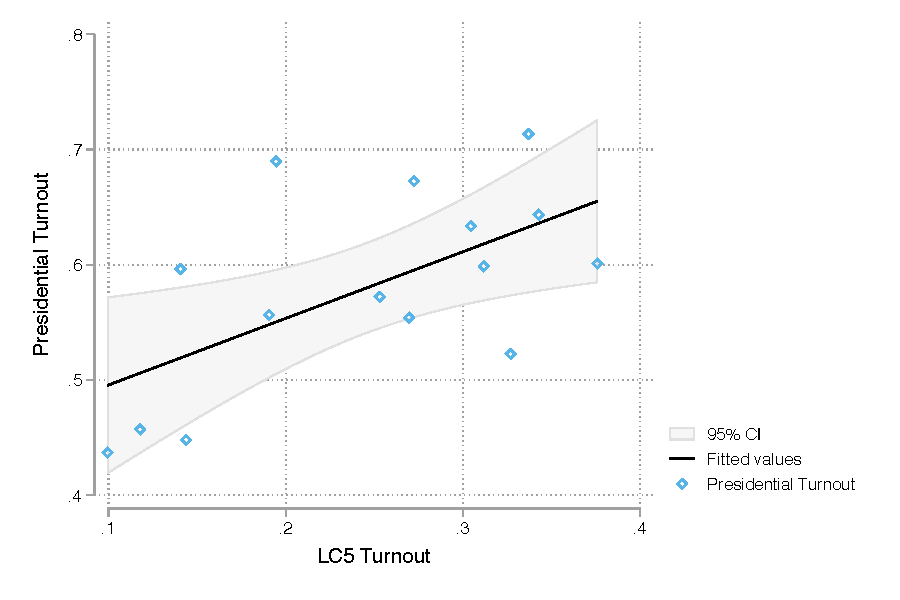
\includegraphics[width=0.6\textwidth]{../3_results/summary_turnout.pdf}
   \end{center}
\end{figure}
\end{samepage}
\fi
%
%\clearpage
\subsection{Simulating Social Context Dynamics}\label{section_simulation}

Social context theory is premised on the assumption that individuals are more likely to participate politically if their peers do so. To understand the dynamics of how this assumption shapes behavior on different types of networks, we use a slightly modified version of the simulation model of \cite{Siegel:2009vi}, which is substantively analogous to \cite{Rolfe:2012ka}. Details of our small technical modification to \cite{Siegel:2009vi} can be found in Appendix~\ref{appendix_tpp_notes}.

The starting point of the simulation is that vertices $v \in V$ in a network choose whether or not to participate in a political activity. Initially, the simulation begins with all vertices endowed with some {\it individual} proclivity to participate. All vertices are assumed to begin in a state of non-participation at $t=0$, but in the first stage, vertices (or nodes) with very high individual proclivities begin to participate. In each state of the simulation, vertices observe the behavior of {\it only} their peers and then decide whether to  participate. A vertex decision to participate is increasing in the share of her peers that are participating. %Similarly, an individual surrounded by non-participants becomes less likely to participate.
The simulation then continues this cycle of vertices observing their peers, updating their own behavior, then observing their peers once more until the network converges to a stable configuration in which behavior no longer changes between stages. More specifically, the simulation proceeds as follows:

\emph{Model Initialization: $t=0$}
	 \begin{itemize}
 	  	\item Vertices are randomly assigned an individual propensity to participate $\beta_v\sim Normal(\beta_{mean}, \beta_{sd})$. Once assigned, these values are fixed for the duration of the simulation.
 		  \item All vertices begin in a state of non-participation ($participation_{v,0} = 0 \, \forall v \in V$)
	  \end{itemize}
\emph{Social Influence Simulation: $t\geq 1$}
	   \begin{itemize}
        \item At each step of the simulation $t \in T$, each vertex $v \in V$ updates its decision about whether to participate based on the decision rule:  $participation_{v,t} = 1$ if $\beta_v - (1-lpr_{v,t-1}) > 0$. $lpr_{v,t-1}$ is the \emph{local participation rate} at time $t-1$: the share of the people connected to $v$ in the network who were participating at time $t-1$.
        \item Overall ``Theoretically-predicted Political Participation'' is then calculated as $TPP_t = \frac{\sum_{v}^V participation_{v,t}}{|V|}$.
        \item The simulation continues until the value of $TPP$ converges.
    \end{itemize}



Several aspects of this framework are worth noting. First, individuals with high values $\beta$ (specifically, $\beta > 1$) will participate politically \emph{even if none of their immediate neighbors plan to participate.} Similarly, individuals with very low values of $\beta$ ($\beta < 0$) will never participate, even if all of their peers are participating. For anyone with a value of $\beta \in (0, 1)$, there is a threshold level of peer participation that will induce those individuals to participate. For example, if $\beta_v = 0.5$, then $v$ will participate if and only if at least  half of her friends participate.

The second aspect of this model is that it is %generally
dynamic. We begin in a state of non-participation at time $t=0$, then in the first period only people with $\beta > 1$ will participate. But as people with $\beta > 1$ announce they are participating, that changes the value of $lpr$ for everyone connected to one of these rabble-rousers, potentially leading them to plan to participate as well. These spillovers may---but also may not, {\it depending on network structure}---cascade for a period of time before eventually the network stabilizes into an equilibrium level of political participation, which may occur at any level between no one participating and everyone participating.

The focus of our analysis is on the average level of political participation to which this model converges for given values of $\beta_{mean}$ and $\beta_{sd}$ -- what we term Theoretically Predicted Participation (TPP). TPP is calculated by simulating this process of influence repeatedly on the network of each village until the simulation converges, then calculating the average level of participation at these convergent states. In other words, TPP is a network structure property. For a given pair of parameters $\beta_{mean}$ and $\beta_{sd}$, villages whose networks converge to higher levels of {\it simulated} participation (higher TPP) %than the network of another village, then our theoretical prediction is that the village that converged to higher levels of political participation
should also have higher levels of {\it actual} (observed) voter turnout.

%\subsection{TPP and Network Structure}

Importantly, the use of simulations is motivated by the fact that whether a network will support a ``snowballing'' of social influence or not has no mechanical relationship to basic network properties (like average number of connections or degree distribution). This is because in a social context model, adding connections among individuals doesn't just increase exposure of individuals to rabble rousers (which will increase an individual's likelihood of participating); it also increases exposure to non-participants (which will depress participating). In a simulation where rabble rousers are relatively rare, for example, participation will only snowball if the network has small pockets where these rabble rousers constitute a large portion of the local neighborhood, making it possible for them to have sufficient influence to induce others in their pocket to participate, generating a critical mass of participants. In a fully connected network, if rabble rousers are rare globally, they will also be rare in every local neighborhood, and thus will never induce increased participation. It is for this reason that small-world networks are often most supportive of high equilibrium TPP \cite{Siegel:2009vi}. The only way to know if political participation will spread on a network, therefore, is through simulation.

Of course, this is not to say that different network properties may not be highly correlated. Indeed, in our data, the correlation between average degree and index of simulated equilibrium participation turns out to be      0.98 for the Union network. But it is worth emphasizing that this is an empirical regularity in these networks, not a relationship that is intrinsic to the measure as past work has shown \citep{Siegel:2009vi}.\footnote{Indeed, it is quite easy to construct networks that not only have the same average degree, but also identical degree distributions with very different TPP scores due to differences in network topology.} As such, it is only because we simulated TPP on these networks that we are aware of this strong empirical relationship. If replicated in other social network data sets, this suggests that real-world social networks tend to have topologies in which average degree is related to ability to support participation snowballs, a finding which would have important implications for the interpretation of analyses of average degree.

\subsection{Simulation Result Summary}

We focus on parameter values of $\beta_{mean} \in \{0.5, 0.6, 0.7\}$ and $\beta_{sd} \in \{0.25, 0.5\}$. These parameter values are chosen because they effectively cover the entire range of values that give rise to interesting dynamics in our networks. Significantly higher values of $\beta_{mean}$ tend to result in convergence to full participation, while substantially lower values lead to non-dynamic simulations (those with values of $ \beta > 1$ participate, but they are rare and others tend to have very low proclivities to participate, as a result of which almost no vertices flip from non-participation to participation). Similarly, larger values of $\beta_{sd}$ increase the share of individuals whose behavior is unaffected by the behavior of other so much that the simulations tend not to be dynamic. In these non-dynamic settings, all networks are essentially comparable, as participation ends up being roughly equal to the share of nodes with $\beta_{mean} > 1$, which is the same for all networks in expectation. Note that we exclude one parameter pair from those sets ($\beta_{mean}=0.5, \beta_{sd}=0.25$), as it generates almost no unconditional participators, and thus no dynamics.

Average TPP scores across study area villages for different parameter values and network specifications are presented in Table~\ref{average_tpp}. Moreover, the inter-village correlation in TPP scores across this parameter space is quite high, as shown in Tables~\ref{corr_union}-\ref{corr_solver} in Appendix~\ref{appendix_socialcontext_validity}. The overall average correlation across parameters for the Union network is      0.64\unskip, and so for ease of exposition (and to reduce the number of regressions we run on the same data), most of the following results will be presented using an index constructed as the first principle component of these statistics for each network type.

\begin{table}
		\begin{center}
			\caption{Average Theoretically-Predicted Participation (TPP)}\label{average_tpp}
		    \begin{tabular}{rrrrr}
\toprule
 $\beta_{mean}$ &  $\beta_{sd}$ &  Mean, Union &  Mean, Family &  Mean, Friends \\
\midrule
           0.50 &          0.50 &         0.42 &          0.39 &           0.36 \\
           0.60 &          0.50 &         0.67 &          0.59 &           0.54 \\
           0.60 &          0.25 &         0.45 &          0.38 &           0.30 \\
           0.70 &          0.50 &         0.83 &          0.77 &           0.71 \\
           0.70 &          0.25 &         0.98 &          0.96 &           0.89 \\
\bottomrule
\end{tabular}

		\end{center}
		\scriptsize{\emph{Notes:}  This table presents average simulated TPP levels across villages for different parameter values and network specifications. Correlations between village TPP scores across different parameters can be found in Appendix~\ref{appendix_socialcontext_validity}.}
\end{table}


\section{Social Context and Turnout}\label{section_results}

Figure~\ref{figure_social_context_scatter} presents the bivariate correlation between the TPP (operationalized as the first principle component of normalized TPP scores across all parameter choices) and actual turnout in the Presidential and district (LC5) elections for the Union network. Note that while TPP is surely estimated with some measurement error, as it enters into our regressions as an independent variable, this will only result in attenuation bias, generating conservative estimates of statistical significance. Regression tables and results for separate network types can be found in Appendix~\ref{appendix_core_result_by_network_type}.

First, in both LC5 specifications, TPP is positively correlated with turnout. Second, the results are significant, despite our relatively small sample size, attenuation bias from measurement error in estimation of TPP, and noise in our dependent variable introduced from estimating voter turnout (which will also depress significance). Moreover, the correlation between these factors appears relatively uniform --- results are not being driven by outliers, as is the risk in small-N studies --- and the relative consistency across specifications provides further evidence of a genuine relationship.

These correlations are also robust to the introduction of different controls and sample restrictions. As shown in Appendix~\ref{appendix_robustness}, results are unchanged when controlling for ethno-linguistic fractionalization or the share of each village that has completed primary school, or when restricting the sample to the set of villages for which our estimates of turnout are likely most accurate. Point estimates are also very stable (albeit not significant) when controlling for network size and when including the exceptionally small 16th village and controlling for size. Finally, results are similar when allowing for only reciprocated friend and family ties, although as discussed in Appendix~\ref{appendix_reciponly}, the low degree count for reciprocated family and friend networks means this is not our preferred specification.\footnote{The average person in our survey has 0.3 reciprocated friends, and 1.5 reciprocated family ties, suggesting limits placed on the number of reportable names resulted in under-reporting of reciprocations.}

\vspace*{-0.1cm}
\begin{figure}
	\begin{center}
	    \caption{}\label{figure_social_context_scatter}
    		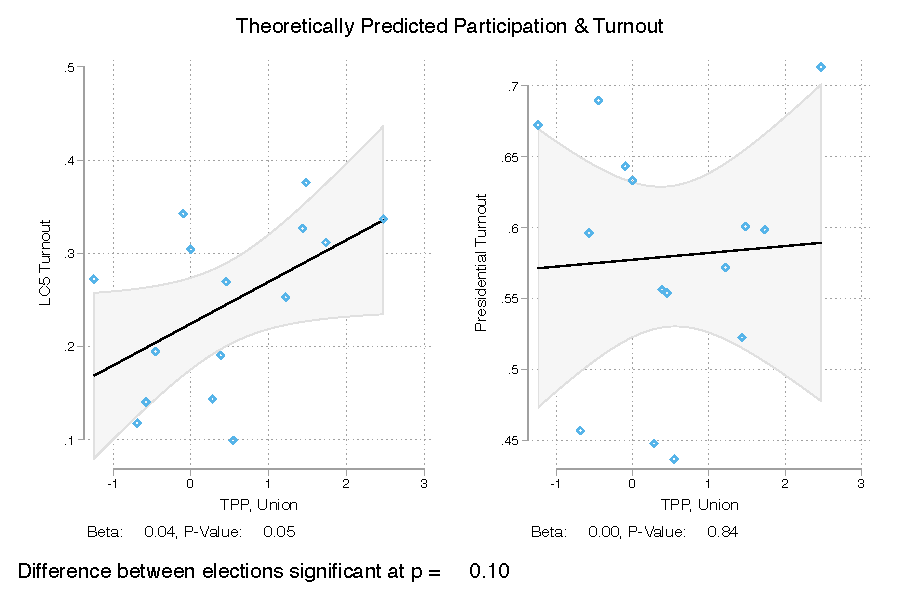
\includegraphics[width=\textwidth]{../3_results/context_voting_scatter.pdf}
    \end{center}
	\scriptsize{\emph{Notes:}  The plot presents the partial correlation between Theoretically-Predicted Participation (TPP) and voter turnout in the Ugandan Presidential and LC5 Chair Elections.  Grey bands indicate 95\% confidence intervals.  As detailed in Section~\ref{section_simulation}, TPP is operationalized as the first principle component of normalized TPP scores across all parameter choices (as TPP is highly correlated across parameters). Turnout is measured as a share of the adult village population. Regressions corresponding to these plots, as well as tests for the statistical significance of differences across elections can be found in Appendix~\ref{appendix_core_result_by_network_type}, along with analogous plots for different sub-networks. Adjustments for measurement /estimation error in TPP have not been made in these estimates; as a result their statistical difference from zero is likely under-stated, as measurement error in independent variables results in attenuation bias.}
\end{figure}

We interpret the correlation in the LC5 elections as support for network structure theories of social influence. Moreover, we suspect the difference in results between the presidential election and the LC5 election may relate to media environments. In Uganda, the presidential election is a much higher-salience election that garners substantially greater media attention and entails far more campaign efforts. It seems likely that voters are exposed to information about the likelihood that peers and non-peers will turn out from many non-network channels, such as election rallies. As a result, the specific topology of village networks should matter less for shaping the social contexts that influence voter turnout decisions.  As demonstrated in the right-hand panel of Figure~\ref{figure_social_context_scatter}, this is what we find, though the correlation is still in the predicted direction. In the lower-salience LC5 election, by contrast, a larger share of the information voters receive about anticipated participation likely comes through their day-to-day interactions and conversations, which are largely dictated by their social networks, increasing the observed correlation between network structure and turnout.\footnote{An alternative explanation for the difference between local and presidential elections is that there are ceiling effects in the latter. As shown in SI, Figure \ref{figure_adultturnout}, turnout in the presidential race in our sample ranges from        44\unskip\% to         71\unskip\% of the adult population, and        51\unskip\% to        77\unskip\% of registered voters, far below the point where we would expect ceiling effects to operate. The national average turnout was 68 percent of registered voters.}

Of course, this is not the only possible explanation for this pattern. The higher salience of the presidential election may also result in voters being less influenced by social context and more influenced by their own political views (i.e. there may be a higher $\beta_{sd}$ for that election), an explanation that would also have important implications for the scope conditions of future studies of network influence. Further research will be required to learn whether this result is generalizable, and if so, what is its exact cause.

To push forward our understanding of how TPP might matter for turnout, we examine heterogeneous effects of social context in more and less competitive elections and where there is greater and lesser variation in the distribution of votes across candidates. These analyses are suggestive, as our sample size of fifteen village puts severe constraints on statistical power for subgroup analysis. First, as shown in SI Table~\ref{table_heterogeneous_by_blockvoting} we find that social context effects are somewhat smaller in villages where voters' candidate preferences are more homogeneous. Second, while the effect of TPP is slightly larger among villages with more competitive down-ballot LC3 local elections, there is no evidence of a heterogeneous impact of TPP for villages facing more competitive down-ballot LC5 council seat elections.\footnote{LC5 Chairs are elected at the County level, regular LC5 Councilors are elected at the Sub-County level, offering variation across villages. LC3 councilors are elected at the even lower Parish level.} While only suggestive (given our limited statistical power), taken together these results point towards network effects supporting a social norm of political participation, rather than facilitating strategic mobilization around a certain party or candidate.


\section{Other Forms of Political Participation}\label{section_other_political_participation}

While the focus of much research on social influence and networks has been on voter turnout, social context theory is generally agnostic about the specific form of social behavior being fostered. For example, a classic example of social context mirror comes from the increased likelihood of individuals to give money to street buskers when a confederate gives in front of them \citep{Cialdini:2015gt}. With that in mind, we further examine the relationship between TPP and self-reported information on participation in village governance. In particular, we find that TPP correlates with (a) the share of villagers reporting having attended a village meeting and (b) the share who report having contributed (in time, cash, or labor) to a village project. These results are presented in Figure~\ref{figure_otherparticipation}. Consistent with theory, we find that our correlation between political participation and TPP holds up for these alternate behaviors, providing two additional data points in support of social context theory. In addition, in the case of meeting attendance, the correlation is quite strong and significant despite the relative small sample size and attenuation bias from measurement error in TPP.

\begin{figure}[!h]
	\begin{center}
	    \caption{}\label{figure_otherparticipation}
    		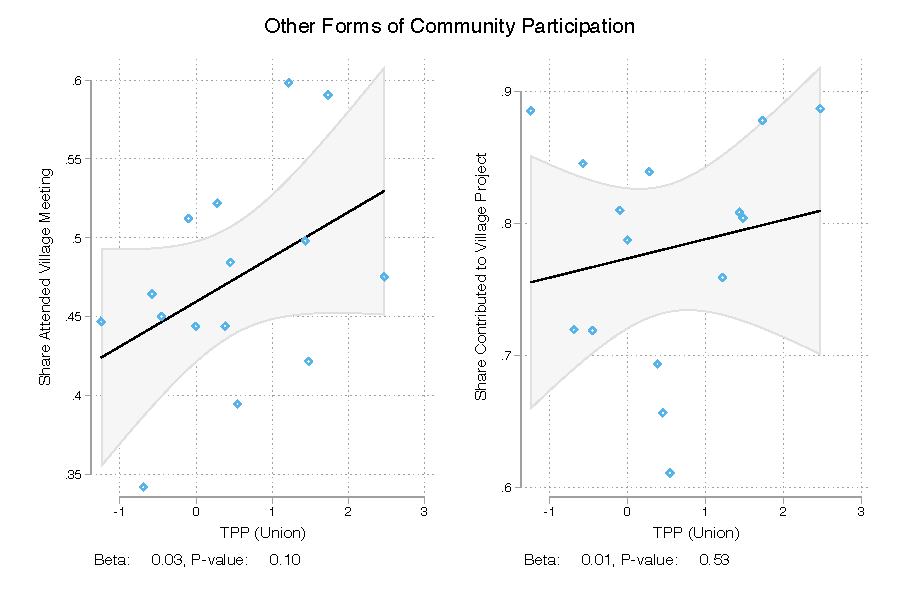
\includegraphics[width=\textwidth]{../3_results/network_and_other_participation}
    \end{center}
	\scriptsize{\emph{Notes:}  The above plot presents the partial correlation between Theoretically-Predicted Participation (TPP) and two alternate forms of political participation: attendance at village meetings and contributions to village projects. Grey bands indicate 95\% confidence intervals. As detailed in Section~\ref{section_simulation}, TPP is operationalized as the first principle component of normalized TPP scores across all considered simulation parameters (as TPP highly correlated across parameters). Data on attendance and contributions is self-reported. Adjustments for measurement /estimation error in TPP have not been made in these estimates; as a result their statistical difference from zero is likely under-stated, as measurement error in independent variables results in attenuation bias.}
\end{figure}

\section{Alternate Explanations}

We briefly address three alternative explanations for the observed correlation between TPP and voter turnout: (a) that the relationship is spurious and should be attributed to differences in pro-social norms; (b) that TPP simply captures mobilization efforts of central agents; and (c) that networks matter for disseminating information on elections, rather than on the voting intention of peers. We rule out these explanations in turn.

%Specifically, we test whether (a) both networks and turnout are shaped by a third factor like pro-social norms, (b) differences in network structure are driven by the presence of ``brokers'' who may facilitate mobilization, and (c) differences are driven by the capacity of networks to diffuse information increasing awareness of the election. We find no support for these alternate explanations.

\subsection{Differences in Pro-Social Norms}

A common concern in observational network studies is that an unobserved third factor is driving both the behavior being measures and network structure. For example, one might worry that communities consisting of more pro-social individuals also tend to form networks with high TPP values, and are more likely to participate politically. We test for this directly using behavioral games conducted as part of a ``lab-in-the-field'' component of the survey from which this network data is drawn. In particular, we test whether villages with higher TPP are also villages in which participants are more other-regarding as measured in a divide-the-dollar dictator game.\footnote{See Appendix~\ref{appendix_divide_the_dollar} for game details.} If pro-sociality is driving both network structure and turnout, generosity in the divide-the-dollar game should be positively correlated with TPP. As shown in Figure~\ref{figure_generosity}, however, if anything, there is a \emph{negative} correlation between pro-sociality among lab subjects and TPP.

\begin{figure}[!h]
	\begin{center}
	    \caption{}\label{figure_generosity}
    		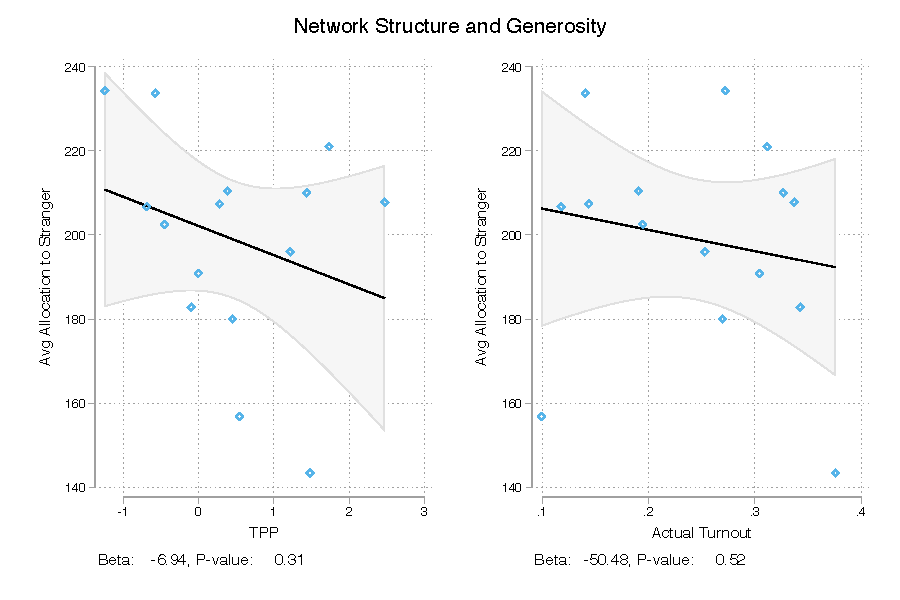
\includegraphics[width=\textwidth]{../3_results/games_and_network.pdf}
    \end{center}
	\scriptsize{\emph{Notes:}  The above plot presents the partial correlation between generosity and turnout (left) and TPP (right). Generosity is operationalized as the portion of ten 100UGX coins subjects agree to give to a randomly selected but unidentified village resident in a lab-in-the-field divide-the-dollar dictator game.  Grey bands indicate 95\% confidence intervals. As detailed in Section~\ref{section_simulation}, TPP is operationalized as the first principle component of normalized TPP scores across all considered simulation parameters (as TPP highly correlated across parameters). Adjustments for measurement /estimation error in TPP have not been made in these estimates; as a result their statistical difference from zero is likely under-stated, as measurement error in independent variables results in attenuation bias.}
\end{figure}

%As shown in Figure~\ref{figure_generosity},

In addition, we also find that higher turnout is correlated with high TPP when we look only at the network formed by family connections (Appendix~\ref{appendix_core_result_by_network_type}). As family connections are less likely to have been forged in response to an unobserved third factor (like pro-sociality), we take this as additional evidence that it is network structure that is driving this relationship.

\subsection{Role of Central Actors}\label{section_centralactors}

Are differences between the networks in our study driven by the mobilization efforts of central actors? To examine this, we drop the five people with the highest eigenvector centrality from each network. If variation in our measure of TPP were being driven by the presence of a few highly central brokers in some networks, then we would expect the correlation between turnout and this modified TPP to decrease. Instead, as shown in Figure~\ref{figure_context_voting_scatter_drop5}, our LC5 results are strengthened and presidential results remain in the correct direction, indicating that the results are driven by general network structure rather than a small number of facilitators.\footnote{We employ this strategy rather than regressing turnout on the eigenvector centrality scores of the top five people in each village to avoid the difficulty of comparing eigenvector centrality scores across networks. Eigenvector centrality is fundamentally a measure of \emph{relative} centrality among the vertices of a given network, making interpretation of direct (cardinal) comparisons of centrality scores across networks problematic.} Notably, results are similar after dropping the 10 and 15 most connected nodes, as shown in in Appendix~\ref{appendix_dropping_highest}.

\begin{figure}
	    \caption{}\label{figure_context_voting_scatter_drop5}
    		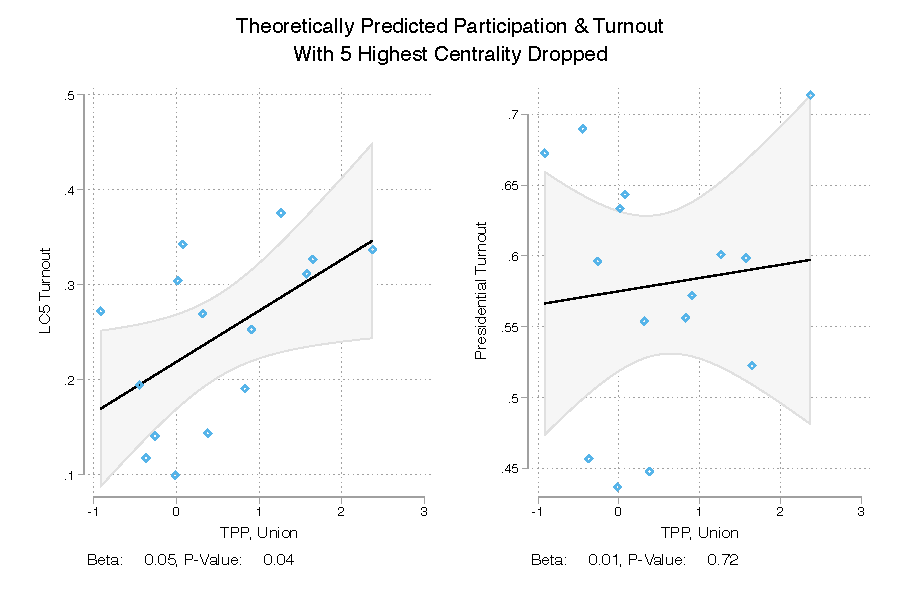
\includegraphics[width=\textwidth]{../3_results/context_voting_scatter_drop5.pdf}
	\scriptsize{\emph{Notes:}  The above plot presents the partial correlation between voter turnout in the Ugandan Presidential and LC5 Chair Elections and a modified version of TPP.  Grey bands indicate 95\% confidence intervals. In particular, TPP has been re-calculated by removing the five individuals with highest eigenvector centrality from each network and re-running TPP simulations on those networks.}
\end{figure}


%Figure~\ref{figure_context_voting_scatter_drop5} plots turnout and TPP \emph{after}

\subsection{Information Diffusion}

A final concern is that networks that give rise to higher TPP may also be networks that better support the efficient diffusion of information, leading to greater turnout. In other words, one might imagine that the role of the social network has little to do with the social context model, but instead with the diffusion through the social network of information, for example about the time and place of the local election, or candidates' policy platforms.

We offer two tests of this possibility. First, we correlate awareness of the UBridge program with TPP. UBridge was a novel program introduced by USAID to a number of individuals within each village. If the efficiency by which networks diffuse information is driving our results, then UBridge awareness and TPP should be positively correlated. As shown in Figure~\ref{figure_ubridge_turnout}, they are not. Moreover, as shown in Appendix~\ref{appendix_inforegs}, TPP remains a significant predictor of turnout even when regressing turnout on TPP and UBridge awareness.



\begin{figure}[!h]
    \caption{UBridge Awareness \& TPP}\label{figure_ubridge_turnout}
    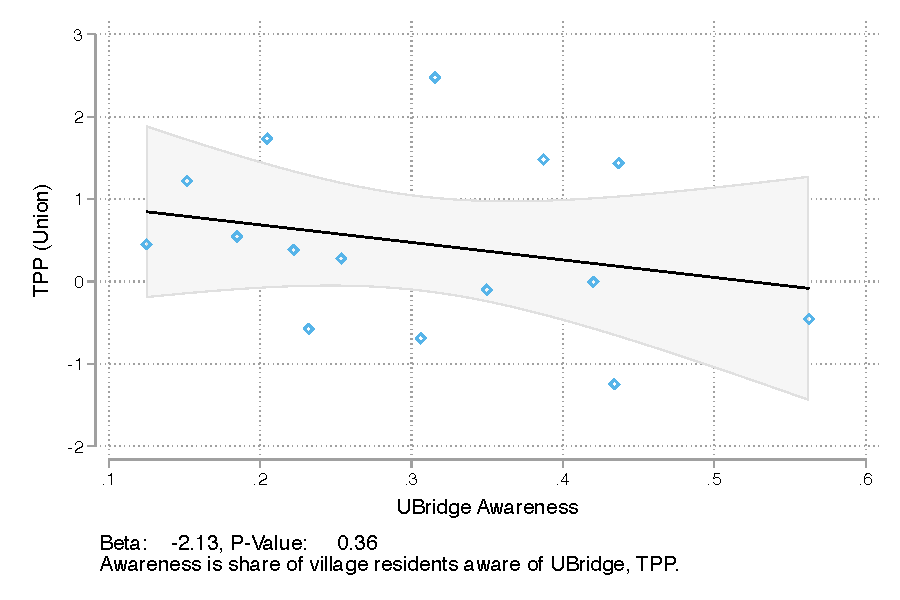
\includegraphics[width=\textwidth]{../3_results/ubridge_awareness_tpp.pdf}
	\scriptsize{\emph{Notes:} The above plot presents the partial correlation between the share of each village that reports awareness of the UBridge program in household surveys and TPP.  Grey bands indicate 95\% confidence intervals. As detailed in Section~\ref{appendix_diffusion_model}, TPP is operationalized as the first principle component of normalized TPP scores across all simulation parameters. Adjustments for measurement /estimation error in TPP have not been made in these estimates; as a result their statistical difference from zero is likely under-stated, as measurement error in independent variables results in attenuation bias.}
\end{figure}

Second, we take advantage of the fact that the properties of networks that support information diffusion are quite distinct from the properties that support high participation in social context models, allowing for easy differentiation of these mechanisms.\footnote{The reason is similar to the reason that average degree is not a robust predictor of equilibrium participation in social context models across different network topologies. Consider a fully connected network. This network will diffuse information quickly, but may not support high TPP. This is because when rabble rousers are relatively rare, participation will only increase if the network has small pockets where these rabble rousers constitute a large portion of the local neighborhood, making it possible for them to have sufficient influence to induce others to participate. In a fully connected network, if rabble rousers are rare globally, they will also be rare in every local neighborhood, and thus will never induce increased participation.} This makes it possible to create an empirically distinct measure of each village network's ability to support information diffusion via simulation. In particular, we operationalize ``diffusion efficiency'' as the average share of each village reached within a given number of steps of a diffusion simulation (see Appendix~\ref{appendix_diffusion_model} for more details).

As shown in Figure~\ref{figure_info_diffusion_turnout}, we find diffusion efficiency is uncorrelated with TPP. And as with UBridge awareness, TPP remains a significant predictor of turnout even when regressing turnout on TPP and information diffusion efficiency (Appendix~\ref{appendix_inforegs}).


\begin{figure}[!h]
    \caption{Simulated Information Diffusion and TPP}
    \label{figure_info_diffusion_turnout}
    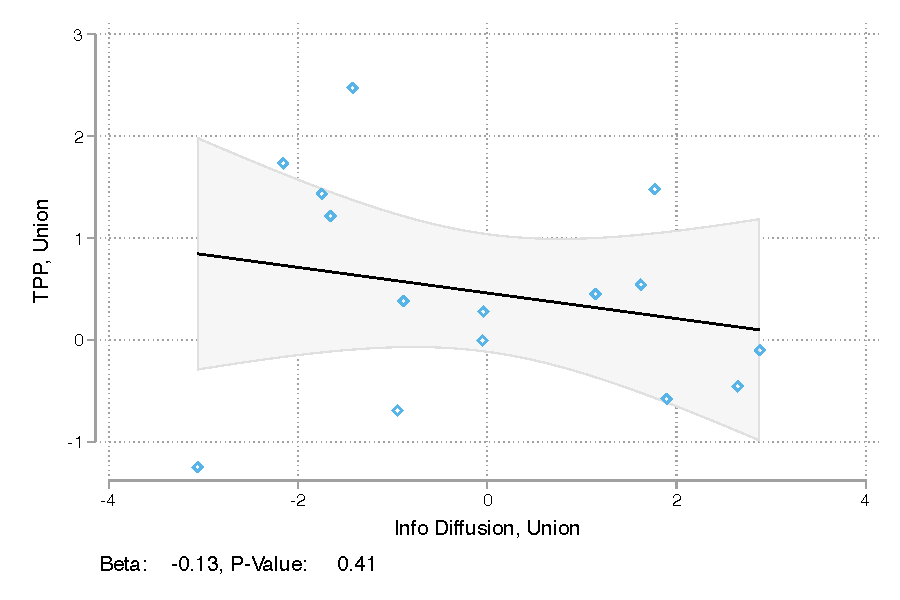
\includegraphics[width=\textwidth]{../3_results/info_and_tpp_scatter.pdf}
	\scriptsize{\emph{Notes:} The above plot presents the partial correlation between the simulated information diffusion efficiency with which village networks diffuse information and TPP. Grey bands indicate 95\% confidence intervals.  As detailed in Section~\ref{appendix_diffusion_model}, diffusion efficiency is operationalized as the first principle component of normalized diffusion rates across a number of simulation parameters, analogous to the operationalization of TPP. Adjustments for measurement /estimation error in diffusion efficiency have not been made in these estimates; as a result their statistical difference from zero is likely under-stated, as measurement error in independent variables results in attenuation bias.}
\end{figure}

\section{Conclusions}

This study provides, to the best of our knowledge, the first direct, empirical test of the theoretical predictions of social context theory, which hitherto was only substantiated using simulated (as compared to real-world) data. It finds that at least among the 15 Ugandan villages examined herein, the theoretical predictions of \cite{Siegel:2009vi} and \cite{Rolfe:2012ka} on how network structure may impact political participation are borne out.

In addition to providing the first test of these theories based on real-world rather than simulated network data, our exercise offers several important lessons for political science theories that take seriously the role of social networks. Most importantly, it suggests that the importance of networks may be contingent on the environment being studied. In particular, our results suggest that in contexts where individuals exposed to extensive messaging by extra-network mediums, the influence of network dynamics may be diminished. Of course, in a single study we cannot show with certainty that this the reason for our heterogeneous results.  It is also possible that voters care more about the presidential elections, and as a result their behavior may be less influenced by that of their peers. Nevertheless, these results point to possible directions for future research, as they suggests an important scope condition for studies of network influence of the type characterized by \cite{Rolfe:2012ka} and \cite{Siegel:2009vi}. Peer-to-peer networks may matter tremendously for political participation related to less high-profile elections or causes, but less so for those that are covered extensively by public media.

However, another interpretation of our result is that the \emph{relevant} sources of social influence might vary across contexts. Here, we believe that for the presidential election the relevant source of influence was likely rallies and mass media, while for the LC5 elections it was peer networks. A similar principle may apply not just in different contexts, but also for demographic groups:  in a given rural US community, the relevant source of influence for older Americans may be their in-person peer networks (or the evening news), while for younger residents it may be social media networks. In other words, one interpretation of our result might be that ``the \emph{relevant} network of social influence is likely to vary across contexts,'' rather than ``sometimes networks of social influence matter and sometimes they don't.''

This analysis also points to the promise of using rich empirical measures to differentiate between mechanisms of network influence, and the promise of mapping entire networks. Because we use theoretically-motivated measures (like diffusion efficiency and TPP), we are able to move beyond just showing that ``networks matter'' and actually offer empirical evidence to show \emph{why} they matter.  In other ``small world'' social networks around the world, where peer-to-peer networks are likely the most relevant network, otherwise puzzling variation in participation might be explained by the extent to which the network structure helps the local ``rabble rousers'' to extend their influence.  Examples include not only voting in local elections, but also helping with village-level cooperative projects, attending public meetings, and joining social movements.

Finally, our study hints at resolutions to remaining puzzles in the study of social context and turnout.  For instance, differences in turnout between urban and rural voters in local elections may have to do with geographic variation in the structure social networks, or in the relative importance of peer-to-peer networks.  Members of racial minority groups may be more likely to participate when living amongst other minorities because of the social networks in which they are embedded \citep{anoll2018}, and declines in turnout associated with residential moves might have to do with disruptions in the social networks that sustain political participation.  Mapping complete networks is time-consuming and costly, but potentially worth the investment.

\vspace*{-0.4cm}

%\clearpage
\singlespacing
\bibliographystyle{apsr}
\bibliography{uganda_voting_bibtex}
\clearpage

\doublespacing
\begin{appendix}
\section*{Online Appendix}
\setcounter{page}{1}
\section{Network Survey}\label{appendix_surveydetails}
We collect data from a set of Ugandan villages that took part in a multi-year program called Governance, Accountability, Participation, and Performance (\href{https://www.rti.org/impact/uganda-governance-accountability-participation-and-performance-gapp}{GAPP}), which was implemented by \href{https://www.rti.org/}{RTI International} and funded by the United States Agency for International Development (USAID) in Arua district, Uganda. 16 villages were selected from a set of over 131 villages that were part of the U-Bridge program, the maximum number that could be enumerated considering budget constraints. Half of the villages had a relatively high level of adoption of the U-Bridge program given village characteristics, and half of which had low levels of adoption. the process of selecting the highest and lowest performers was as follows. We regressed village level adoption of the U-Bridge technology on village-level predictors, and generate a set of predicted values for the dependent variable. We then calculated the difference between the predicted value and the actual value of U-Bridge adoption. Using these residuals, we selected the 8 highest performing and the 8 lowest performing villages with respect to U-Bridge adoption.

We conducted a census in each village in order to collect complete network data, interviewing every available adult who was a resident in the village. This involved a village listing prior to enumeration, the purpose of which was to create a written record of all of the names and household locations for all adults in the villages. To do this the enumerator met with the village leader (in Uganda, called an LC1) and two other village leaders (usually a member of the Village Health Team and an additional village elder or community leader). Together they drew a map of the village identifying every location of a household and major geographical features (e.g., rivers, churches, etc.). Then the group created a list---using their shared knowledge of those households---to identify and name every adult in the village. The enumerator entered this information into a tablet along with other key identifying information such as quadrant (an arbitrary division of the village created by the enumerator---designed to divide the village into four equal portions), age and gender of the potential respondent. These names were then used in the network section of the survey, where respondents were asked about four types of social ties. The exact question wording for the social ties is as follows:

``In each of the following questions, we will ask you to think about people in your community and their relationships to you.''
\begin{itemize}

\item {\bf Family}: ``Think about up to five family members in this village not living in your household with whom you most frequently spend time. For instance, you might visit one another, eat meals together, or attend events together.''

\item {\bf Friends}:	``Think about up to five of your best friends in this village. By friends I mean someone who will help you when you have a problem or who spends much of his or her free time with you. If there are less than five, that is okay too.''

\item {\bf Lender}: ``Think about up to five people in this village that you would ask to borrow a significant amount of money if you had a personal emergency.''

\item {\bf Problem solver}: ``Imagine there is a problem with public services in this village. For example, you might imagine that a teacher has not come to school for several days or that a borehole in your village needs to be repaired. Think about up to five people in this village whom you would be most likely to approach to help solve these kinds of problems.''
\end{itemize}



\section{Turnout Estimation}\label{appendix_turnout_extrapolation}

As noted above, our turnout measure assumes that votes at a given precinct (polling station) are evenly distributed among voters registered at that precinct from different villages.

To illustrate, assume that at Precinct 1, 200 votes were cast. If 75\% of the voters registered at Precinct 1 come from Village A and 25\% come from Village B, we assume that Village A contributed 150 votes and Village B contributed 50 votes. Turnout for each village is then calculated as the sum of votes we infer to have been case by its residents at all Precincts. By assuming that at a given precinct all villages have the same turnout, this estimation should bias our analysis in favor of \emph{not} finding differences in turnout across villages.

One constraint of this measures is that the accuracy of these estimates will be related to the correspondence of villages to precincts. If each village sends all residents to its own polling place (i.e. that polling place is only attended by residents of one village), inferences about village voting will be perfect. If, by contrast, all villages send their voters to a single polling place, effectively no information can be learned about how individual villages voted.

This correspondence can be summarized using a \emph{concentration} statistic, where higher values mean the mapping from precincts to villages is more precise. For a village $v \in V$ and a polling place (precinct) $p \in P$, let $voters_{v}$ be the set of voters who live in $v$, let $voters_{p}$ be the set of voters who vote at polling place $p$, and let $voters_{v,p}$ be the set of voters who reside in $v$ and voted at $p$. Then:

\begin{equation}
 	concentration_{v,p} \equiv \frac{\#voters_{v,p}}{\#voters_{p}}
\end{equation}

In other words, $concentration_{v,p}$ is the share of voters at a precinct from village $v$.

Since villages send people to multiple polling places, however, we must then calculate a weighted average of $concentration_{v,p}$ across polling places where the weight for each polling place is the share of voters from each village going to that polling place. Formally:

\begin{equation}
	concentration_{v} \equiv \sum_{p \in P} concentration_{v,p} * \frac{\#voters_{v,p}} { \# voters_{v}}
\end{equation}

The distribution of this statistic are presented in Figure~\ref{village_concentration}:

\begin{figure}[bht]
	\begin{center}
	    \caption{Distribution of $concentration_{v,p}$ Measure Across Villages}\label{village_concentration}
    		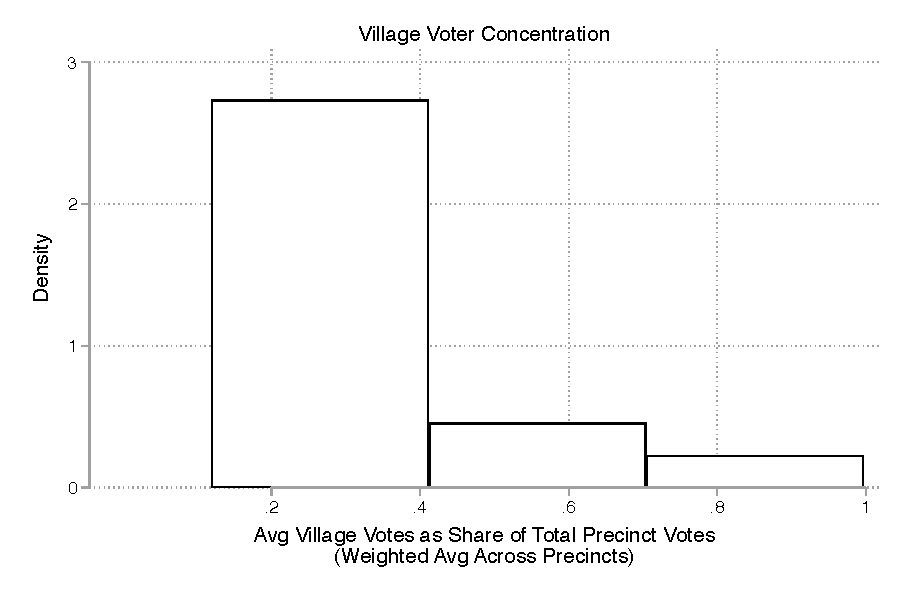
\includegraphics[width=0.5\textwidth]{../3_results/concentration_hist.pdf}
    \end{center}
\end{figure}

Distribution of village-level estimated turnout as share of adult populations are presented below in Figure~\ref{figure_adultturnout}. In addition, we also plot $concentration_{v}$ against TPP in Figure~\ref{figure_concentration_and_tpp}.

\begin{figure}[h!]
  \centering
  \caption{Estimated Village Turnout as a Share of Adult Population}\label{figure_adultturnout}
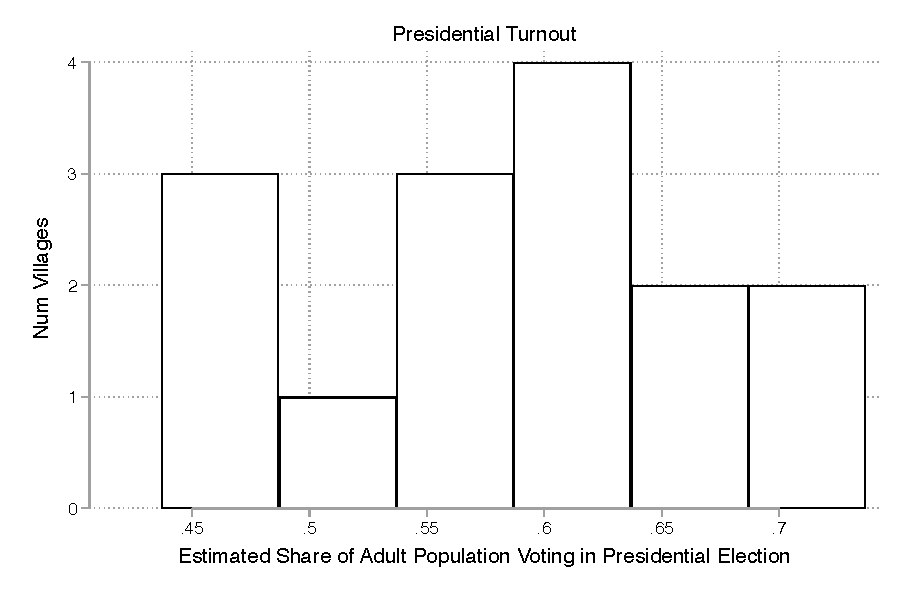
\includegraphics[width=0.45\textwidth]{../3_results/presidential_turnout_hist.pdf}\includegraphics[width=0.45\textwidth]{../3_results/lc5chair_turnout_hist.pdf}
\end{figure}



\begin{figure}[h!]
\begin{center}
  \caption{Precinct / Village Alignment ($concentration_{v}$) and TPP}\label{figure_concentration_and_tpp}
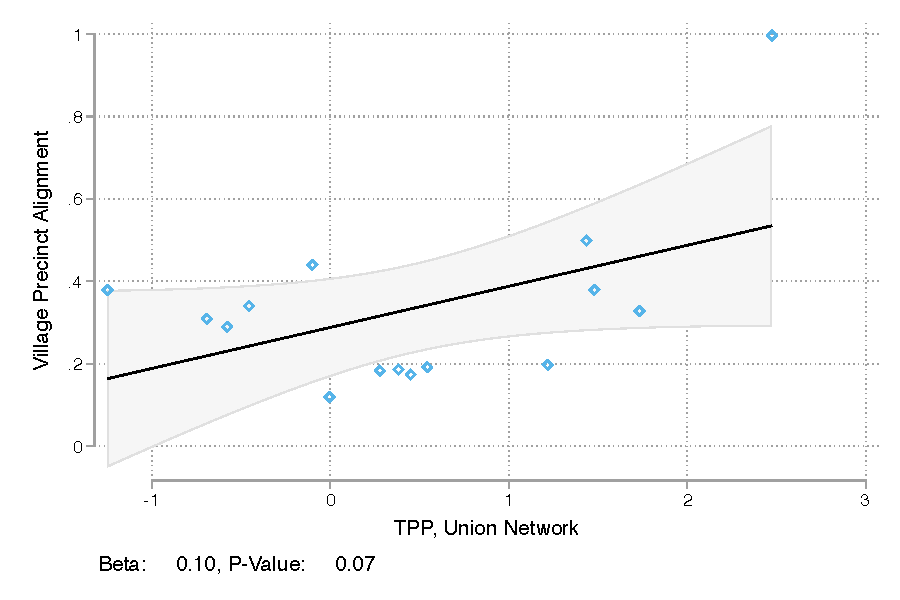
\includegraphics[width=0.45\textwidth]{../3_results/precinct_alignment_pres.pdf}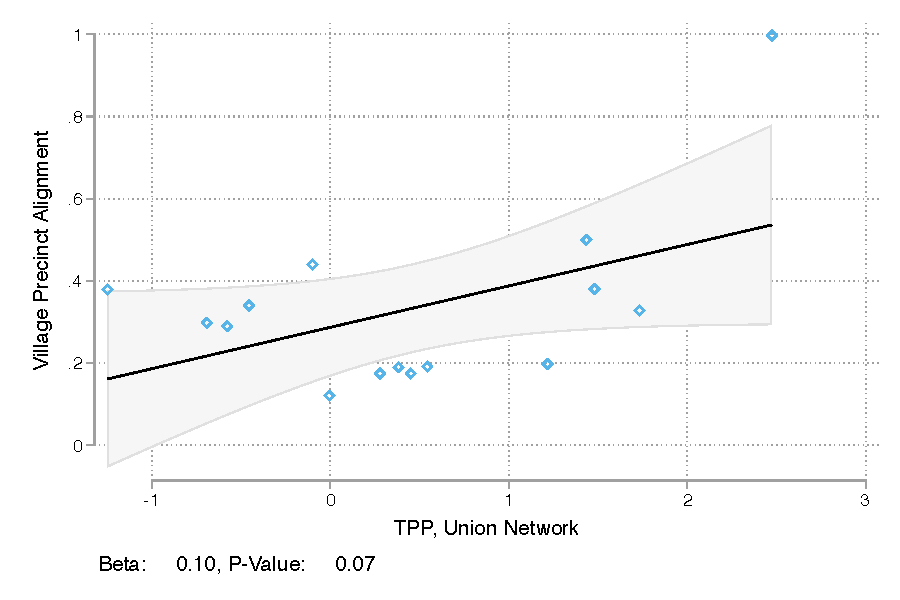
\includegraphics[width=0.45\textwidth]{../3_results/precinct_alignment_LC5chair.pdf}\\
\end{center}
\scriptsize{ \emph{Notes:}  The above plot presents the partial correlation between Theoretically-Predicted Participation (TPP) and precinct / village alignment ($concentration_{v}$). Grey bands indicate 95\% confidence intervals.  As detailed in Section~\ref{section_simulation}, TPP is operationalized as the first principle component of normalized TPP scores across all parameter choices (as TPP is highly correlated across parameters). Presidential and LC5 Chair are concentration are correlated at    0.9998\unskip, which is why the plots are nearly identical.}
\end{figure}


\pagebreak

\section{TPP Simulation Notes}\label{appendix_tpp_notes}


\subsection{Participation Updating}

Updating of the $participation_{v, t+1}$ is accomplished by iterating through all vertices in the network in random order and having each vertex update its value of $lpr$ and its participation $participation_{v, t+1}$ \emph{sequentially} rather than simulatenously. This is the one departure from \cite{Siegel:2009vi}. When all vertices update $lpr$ simultaneously, it is possible to converge to a ``flashing'' state in which at time $t$ a portion of the network is planning to vote while another portion is not planning to vote, at time $t+1$, these two groups flip inclinations, and at time $t+2$ they return to their initial state. This is caused by knife-edge simultaneity of updating, which seems unrealistic, since real updating is almost certainly sequential.  Thus simulation uses sequential updating.

\subsection{Convergence}

The simulation is run until no more than 1\% percent of the vertices in the network change participation status for at least 20 consecutive periods. Results below are averaged across 2,500 runs for each set of parameter values.


\section{Parameter Choices}\label{appendix_parameter_choices}

These parameter values are chosen because they effectively cover the range of values that give rise to interesting dynamics. Significantly higher values of $\beta_{mean}$ tend to result in convergence to full participation, while substantially lower values lead to non-dynamic simulations (those with values of $ \beta > 1$ participate, but they are rare and others tend to have very low proclivities to participate, as a result of which almost no vertices flip from non-participation to participation). Similarly, larger values of $\beta_{sd}$ increase the share of individuals whose behavior is unaffected by the behavior of other so much that the simulations tend not to be dynamic. In these non-dynamic settings, all networks are essentially comparable, as participation ends up being roughly equal to the share of nodes with $\beta_{mean} > 1$, which is the same for all networks in expectation.

Note that we exclude one parameter pair from those sets ($\beta_{mean}=0.5, \beta_{sd}=0.25$), as it generates almost no unconditional participators, and thus no dynamics.


\pagebreak
\begin{landscape}
    \section{Social Context Simulation Validity}\label{appendix_socialcontext_validity}
\begin{table}[htbp]\centering \caption{Correlations across Parameter Values, Union Network\label{corr_union}}
\begin{tabular}{l  c  c  c  c  c }\hline\hline
\multicolumn{1}{c}{Variables} &Mean 0.5, SD 0.5&Mean 0.6, SD 0.5&Mean 0.6, SD 0.25&Mean 0.7, SD 0.5&Mean 0.7, SD 0.25\\ \hline
Mean 0.5, SD 0.5&1.00\\
Mean 0.6, SD 0.5&0.93&1.00\\
Mean 0.6, SD 0.25&0.51&0.56&1.00\\
Mean 0.7, SD 0.5&0.94&0.98&0.55&1.00\\
Mean 0.7, SD 0.25&0.35&0.36&0.84&0.39&1.00\\
\hline \hline 
 \end{tabular}
\end{table}

\begin{table}[htbp]\centering \caption{Correlations across Parameter Values, Family Network\label{corr_family}}
\begin{tabular}{l  c  c  c  c  c }\hline\hline
\multicolumn{1}{c}{Variables} &Mean 0.5, SD 0.5&Mean 0.6, SD 0.5&Mean 0.6, SD 0.25&Mean 0.7, SD 0.5&Mean 0.7, SD 0.25\\ \hline
Mean 0.5, SD 0.5&1.00\\
Mean 0.6, SD 0.5&0.96&1.00\\
Mean 0.6, SD 0.25&0.86&0.89&1.00\\
Mean 0.7, SD 0.5&0.96&0.99&0.86&1.00\\
Mean 0.7, SD 0.25&0.91&0.90&0.83&0.93&1.00\\
\hline \hline 
 \end{tabular}
\end{table}

\end{landscape}
\pagebreak
\begin{landscape}
    \begin{table}[htbp]\centering \caption{Correlations across Parameter Values, Friends Network\label{corr_friend}}
\begin{tabular}{l  c  c  c  c  c }\hline\hline
\multicolumn{1}{c}{Variables} &Mean 0.5, SD 0.5&Mean 0.6, SD 0.5&Mean 0.6, SD 0.25&Mean 0.7, SD 0.5&Mean 0.7, SD 0.25\\ \hline
Mean 0.5, SD 0.5&1.00\\
Mean 0.6, SD 0.5&0.98&1.00\\
Mean 0.6, SD 0.25&0.94&0.98&1.00\\
Mean 0.7, SD 0.5&0.99&1.00&0.97&1.00\\
Mean 0.7, SD 0.25&0.98&0.99&0.96&0.99&1.00\\
\hline \hline 
 \end{tabular}
\end{table}

    \begin{table}[htbp]\centering \caption{Correlations across Parameter Values, Lender Network\label{corr_lender}}
\begin{tabular}{l  c  c  c  c  c }\hline\hline
\multicolumn{1}{c}{Variables} &Mean 0.5, SD 0.5&Mean 0.6, SD 0.5&Mean 0.6, SD 0.25&Mean 0.7, SD 0.5&Mean 0.7, SD 0.25\\ \hline
Mean 0.5, SD 0.5&1.00\\
Mean 0.6, SD 0.5&0.98&1.00\\
Mean 0.6, SD 0.25&0.92&0.97&1.00\\
Mean 0.7, SD 0.5&0.97&0.99&0.97&1.00\\
Mean 0.7, SD 0.25&0.95&0.98&0.97&0.99&1.00\\
\hline \hline 
 \end{tabular}
\end{table}

\end{landscape}
\pagebreak
\begin{landscape}
    \begin{table}[htbp]\centering \caption{Correlations across Parameter Values, Solver Network\label{corr_solver}}
\begin{tabular}{l  c  c  c  c  c }\hline\hline
\multicolumn{1}{c}{Variables} &Mean 0.5, SD 0.5&Mean 0.6, SD 0.5&Mean 0.6, SD 0.25&Mean 0.7, SD 0.5&Mean 0.7, SD 0.25\\ \hline
Mean 0.5, SD 0.5&1.00\\
Mean 0.6, SD 0.5&0.95&1.00\\
Mean 0.6, SD 0.25&0.89&0.95&1.00\\
Mean 0.7, SD 0.5&0.96&0.98&0.96&1.00\\
Mean 0.7, SD 0.25&0.85&0.93&0.92&0.91&1.00\\
\hline \hline 
 \end{tabular}
\end{table}

\end{landscape}
\pagebreak

\section{Turnout and TPP by Network Type}\label{appendix_core_result_by_network_type}

Table~\ref{table_context_voting_regressions} presents the regressions underlying Figure~\ref{figure_social_context_scatter}.

\begin{table}
	\caption{TPP and Turnout Regressions}\label{table_context_voting_regressions}
	{
\def\sym#1{\ifmmode^{#1}\else\(^{#1}\)\fi}
\begin{tabular}{l*{3}{c}}
\toprule
                &\multicolumn{1}{c}{(1)}&\multicolumn{1}{c}{(2)}&\multicolumn{1}{c}{(3)}\\
                &\multicolumn{1}{c}{Presidential}&\multicolumn{1}{c}{LC5 Chair}&\multicolumn{1}{c}{Pooled}\\
\midrule
Eqm Participation Index (Union)&   0.0048         &    0.045\sym{*}  &   0.0048         \\
                &  (0.023)         &  (0.021)         &  (0.026)         \\
LC5 Election * Eqm Participation&                  &                  &    0.040         \\
                &                  &                  &  (0.023)         \\
LC5 Chair Election&                  &                  &    -0.35\sym{***}\\
                &                  &                  &  (0.019)         \\
\midrule
Observations    &       15         &       15         &       30         \\
\bottomrule
\multicolumn{4}{l}{\footnotesize Standard errors in parentheses}\\
\multicolumn{4}{l}{\footnotesize \sym{*} \(p<0.1\), \sym{**} \(p<0.05\), \sym{***} \(p<0.01\)}\\
\end{tabular}
}
 \\
	Pooled estimates clustered at village level.
\end{table}

Figure~\ref{figure_context_friends_family_separately} below shows the relationship between turnout and TPP simulated separately on the four different types of networks that contribute to the Union network presented in the main paper. We find that our main results are generally insensitive to the type of network used to estimate TPP.


\begin{figure}[h!]
	\begin{center}
	    \caption{}\label{figure_context_friends_family_separately}
    		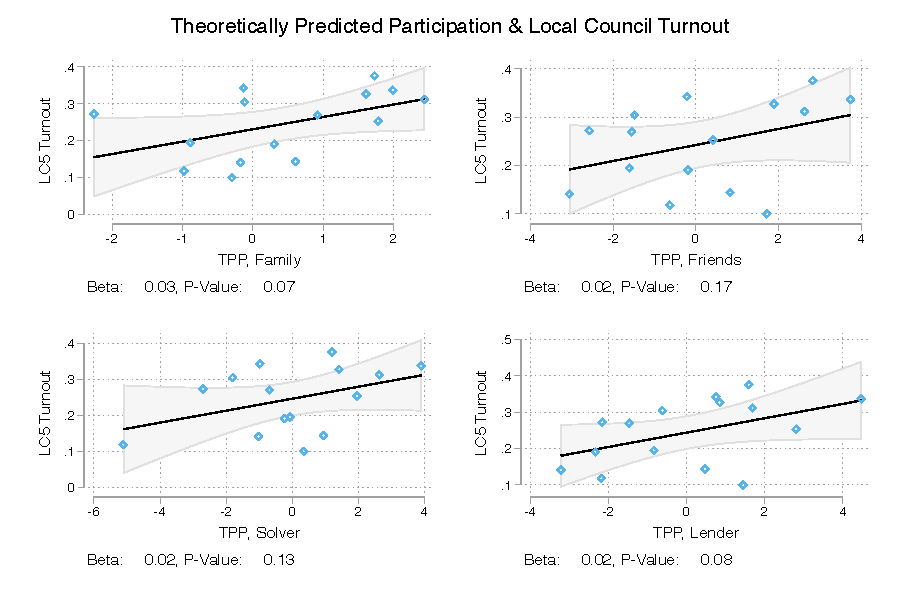
\includegraphics[width=0.8\textwidth]{../3_results/context_voting_scatter_bytype_LC5.pdf}
            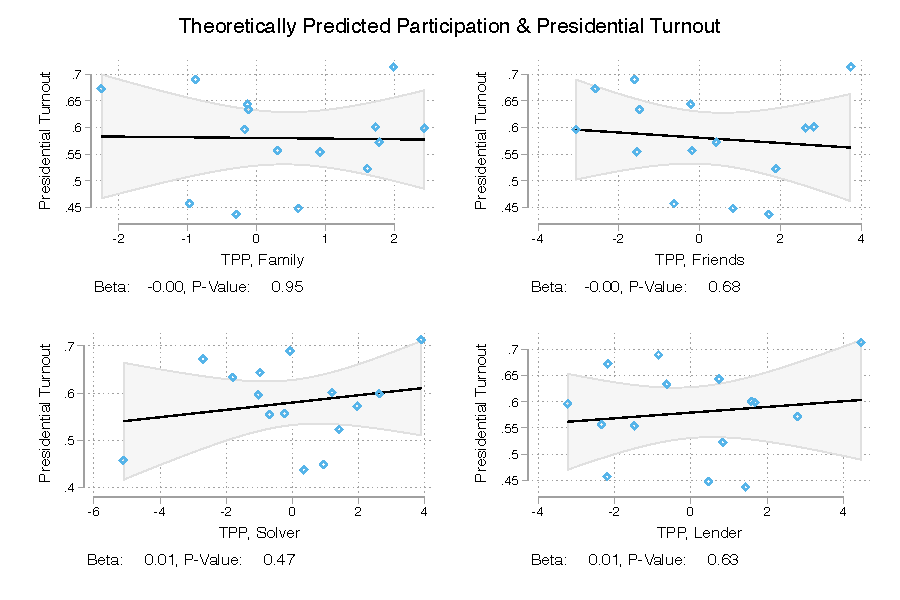
\includegraphics[width=0.8\textwidth]{../3_results/context_voting_scatter_bytype_presidential.pdf}
    \end{center}
\end{figure}
\pagebreak


\section{Robustness Regression Tables}\label{appendix_robustness}
The following tables show robustness of our primary result when controlling for ELF (Column 2), controlling for education (Column 3), subsetting on the half of villages with the best polling-place-village correspondence (Column 4), and when including the exceptionally small 16th village surveyed (Column 5).
\begin{table}[htbp]\centering
\def\sym#1{\ifmmode^{#1}\else\(^{#1}\)\fi}
\caption{Robustness for LC5 Election\label{tablerobustnessLC5chair}}
\begin{tabular}{l*{7}{c}}
\toprule
                &\multicolumn{1}{c}{(1)}&\multicolumn{1}{c}{(2)}&\multicolumn{1}{c}{(3)}&\multicolumn{1}{c}{(4)}&\multicolumn{1}{c}{(5)}&\multicolumn{1}{c}{(6)}&\multicolumn{1}{c}{(7)}\\
                &\multicolumn{1}{c}{Basic}&\multicolumn{1}{c}{ELF}&\multicolumn{1}{c}{Educ}&\multicolumn{1}{c}{Size}&\multicolumn{1}{c}{Concentrate}&\multicolumn{1}{c}{W/16th}&\multicolumn{1}{c}{Village}\\
\midrule
TPP (Union)     &    0.045\sym{*}  &    0.044\sym{*}  &    0.046\sym{*}  &    0.038         &    0.041\sym{*}  &    0.014         &    0.038         \\
                &  (0.021)         &  (0.022)         &  (0.022)         &  (0.028)         &  (0.020)         &  (0.011)         &  (0.029)         \\
ELF             &                  &   -0.068         &                  &                  &                  &                  &                  \\
                &                  &   (0.13)         &                  &                  &                  &                  &                  \\
Educ            &                  &                  &    0.058         &                  &                  &                  &                  \\
                &                  &                  &   (0.19)         &                  &                  &                  &                  \\
(Log) Network Size&                  &                  &                  &    0.060         &                  &                  &    -0.10         \\
                &                  &                  &                  &   (0.17)         &                  &                  &   (0.12)         \\
\midrule
Observations    &       15         &       15         &       15         &       15         &        8         &       16         &       16         \\
\bottomrule
\multicolumn{8}{l}{\footnotesize Standard errors in parentheses}\\
\multicolumn{8}{l}{\footnotesize \sym{*} \(p<0.1\), \sym{**} \(p<0.05\), \sym{***} \(p<0.01\)}\\
\end{tabular}
\end{table}

\begin{table}[htbp]\centering
\def\sym#1{\ifmmode^{#1}\else\(^{#1}\)\fi}
\caption{Robustness for Pres Election\label{tablerobustnesspres}}
\begin{tabular}{l*{7}{c}}
\toprule
                &\multicolumn{1}{c}{(1)}&\multicolumn{1}{c}{(2)}&\multicolumn{1}{c}{(3)}&\multicolumn{1}{c}{(4)}&\multicolumn{1}{c}{(5)}&\multicolumn{1}{c}{(6)}&\multicolumn{1}{c}{(7)}\\
                &\multicolumn{1}{c}{Basic}&\multicolumn{1}{c}{ELF}&\multicolumn{1}{c}{Educ}&\multicolumn{1}{c}{Size}&\multicolumn{1}{c}{Concentrate}&\multicolumn{1}{c}{W/16th}&\multicolumn{1}{c}{Village}\\
\midrule
TPP (Union)     &   0.0048         &   0.0020         &   0.0041         &   0.0016         &   0.0058         &   -0.027\sym{**} &   0.0012         \\
                &  (0.023)         &  (0.023)         &  (0.024)         &  (0.031)         &  (0.026)         &  (0.012)         &  (0.032)         \\
ELF             &                  &    -0.17         &                  &                  &                  &                  &                  \\
                &                  &   (0.14)         &                  &                  &                  &                  &                  \\
Educ            &                  &                  &   -0.036         &                  &                  &                  &                  \\
                &                  &                  &   (0.21)         &                  &                  &                  &                  \\
(Log) Network Size&                  &                  &                  &    0.030         &                  &                  &    -0.13         \\
                &                  &                  &                  &   (0.18)         &                  &                  &   (0.13)         \\
\midrule
Observations    &       15         &       15         &       15         &       15         &        8         &       16         &       16         \\
\bottomrule
\multicolumn{8}{l}{\footnotesize Standard errors in parentheses}\\
\multicolumn{8}{l}{\footnotesize \sym{*} \(p<0.1\), \sym{**} \(p<0.05\), \sym{***} \(p<0.01\)}\\
\end{tabular}
\end{table}

\pagebreak

\section{Considering Non-Reciprocal Ties}\label{appendix_reciponly}

Figure~\ref{figure_context_voting_scatter_reciponly} presents results when networks are created using only reciprocated ties to form Friends and Family ties (note the other two inputs into the Union network -- the Lender / Solver networks -- cannot be restricted in an analogous manner). The figures show results quite similar under this restriction.

As shown in Table~\ref{table_summary_reciponly}, however, it is not clear that these restrictions are reasonable given the low average degree they generate in the Friend and Family networks. This may be due to censoring caused by the limited number of people individuals are allowed to list (5 family members and 5 friends), or failures to recall individuals.

\begin{table}
\centering
\caption{Network Summary Statistics: Including Only Reciprocated Friends and Family Ties }\label{table_summary_reciponly}
\begin{tabular}{lrrrrr}
\toprule
                         &   Union &   Friends &   Family &   Lender &   Solver \\
\midrule
 Average Size            &   210.3 &     210.3 &    210.3 &    210.3 &    210.3 \\
 Average Num Connections &   924.1 &      34.3 &    156.5 &    403.3 &    450.2 \\
 Average Degree          &     8.7 &       0.3 &      1.5 &      3.8 &      4.2 \\
 Min Size                &   160.0 &     160.0 &    160.0 &    160.0 &    160.0 \\
 Max Size                &   283.0 &     283.0 &    283.0 &    283.0 &    283.0 \\
\bottomrule
\end{tabular}
\end{table}


\begin{figure}[h!]
	\begin{center}
	    \caption{}\label{figure_context_voting_scatter_reciponly}
    		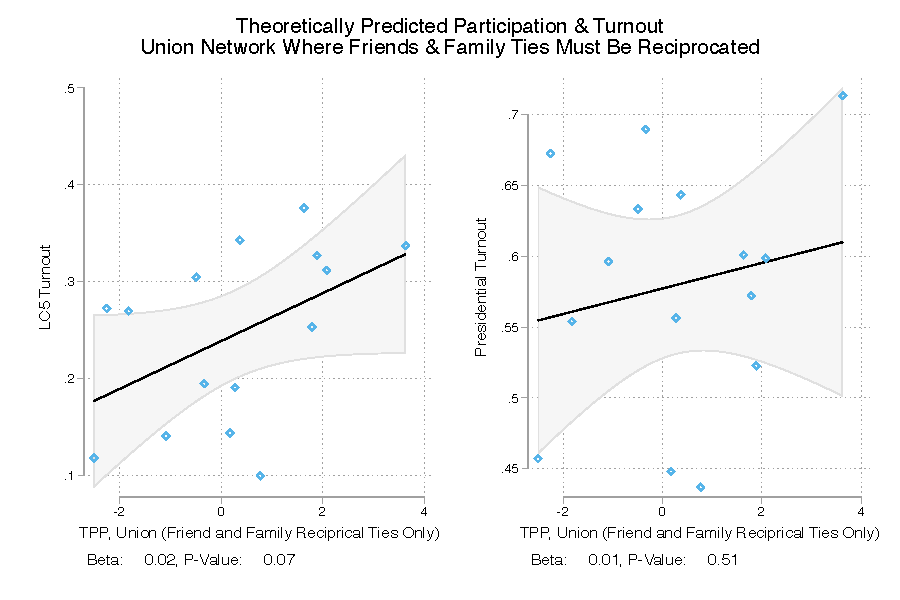
\includegraphics[width=\textwidth]{../3_results/context_voting_scatter_reciponly.pdf}
		\end{center}
			\scriptsize{\emph{Notes:}  The above plot presents the partial correlation between Theoretically-Predicted Participation (TPP) and voter turnout in the Ugandan Presidential and LC5 Chair Elections where ties are only added between friends and family if ties are reciprocated.  Grey bands indicate 95\% confidence intervals.  As detailed in Section~\ref{section_simulation}, TPP is operationalized as the first principle component of normalized TPP scores across all parameter choices (as TPP is highly correlated across parameters). Turnout is shares of the adult village population. Regressions corresponding to these plots, as well as tests for the statistical significance of differences across elections can be found in Appendix~\ref{appendix_core_result_by_network_type}, along with analogous plots for different sub-networks. Adjustments for measurement /estimation error in TPP have not been made in these estimates; as a result their statistical difference from zero is likely under-stated, as measurement error in independent variables results in attenuation bias.}
\end{figure}
\pagebreak

\section{Heterogeneous Effects}\label{appendix_heterogeneous_by_blockvoting}

An important question is whether the social context effects we observe are driven by pressure to vote, or by pressure to coordinate around a given candidate. Table~\ref{table_heterogeneous_by_blockvoting} presents tests for heterogeneous effects of TPP by (a) the degree to which village candidate preferences appear to be homogenous (i.e. everyone votes for the same candidate), and (b) the degree to which down-ballot races are competitive (there is no cross-village variation in the competitiveness of top-of-ticket races).

Vote homogeneity is measured using a simple Herfindahl index (which takes on a value of 1 if everyone votes for the same candidate, and a value of 0 if no one votes for the same candidate), while competitiveness is a fragmentation index (one minus the Herfindahl index of candidate vote shares across their entire electoral district -- a value of 0 for races where one candidate won all votes or stood in an uncontested election, and values approaching 1 where votes are distributed evenly across a large number of candidates).

Note that the results in Column 4-5 are for down-ballot LC5 council seats, which are elected at the Sub-County level, so some villages faced the same slate of candidates. For that reason, results are clustered by sub-county (there are        10 clusters across the 15 villages). Similarly, Column 6 shows the relationship between competitiveness and TPP for down-ballot LC3 races, where villages in the same Parish face the same candidates, so results are clustered by parish (there are        13 clusters across the 15 villages). Column names report the term for the election in which candidates appeared using the election naming convention used throughout this paper (both LC5 council and LC3 candidates stood during the same election in which the LC5 Chair was selected).

First, as shown in Columns 2 and 4, we find that social context effects are somewhat smaller in villages where voters' candidate preferences are more homogeneous. Second, while the effect of TPP is slightly larger among villages with more competitive down-ballot LC3 local elections (Column 6), there is no evidence of a heterogeneous impact of TPP for villages facing more competitive down-ballot LC5 council seat elections (Column 5). While only suggestive (given our limited statistical power), taken together these results point towards network effects supporting a social norm of political participation, rather than facilitating strategic mobilization around a certain party or candidate.

\begin{table}

  \caption{Social Norms and Political Mobilization}\label{table_heterogeneous_by_blockvoting}
  {
\def\sym#1{\ifmmode^{#1}\else\(^{#1}\)\fi}
\begin{tabular}{l*{6}{c}}
\toprule
                &\multicolumn{1}{c}{(1)}&\multicolumn{1}{c}{(2)}&\multicolumn{1}{c}{(3)}&\multicolumn{1}{c}{(4)}&\multicolumn{1}{c}{(5)}&\multicolumn{1}{c}{(6)}\\
                &\multicolumn{1}{c}{Pres}&\multicolumn{1}{c}{Pres}&\multicolumn{1}{c}{LC5Chair}&\multicolumn{1}{c}{LC5Chair}&\multicolumn{1}{c}{LC5Chair}&\multicolumn{1}{c}{LC5Chair}\\
\midrule
TPP (Union)     &   0.0048         &     0.22         &    0.045\sym{*}  &    0.086         &   0.0063         &   -0.052         \\
                &  (0.023)         &   (0.17)         &  (0.021)         &   (0.14)         &  (0.048)         &  (0.046)         \\
Pres Vote Homogeneity&                  &     0.32         &                  &                  &                  &                  \\
                &                  &   (0.25)         &                  &                  &                  &                  \\
TPP X Vote Homogeneity&                  &    -0.42         &                  &                  &                  &                  \\
                &                  &   (0.33)         &                  &                  &                  &                  \\
LC5Chair Vote Homogeneity&                  &                  &                  &    -0.13         &                  &                  \\
                &                  &                  &                  &   (0.19)         &                  &                  \\
TPP X Vote Homogeneity&                  &                  &                  &   -0.086         &                  &                  \\
                &                  &                  &                  &   (0.26)         &                  &                  \\
LC5 Council Competitive&                  &                  &                  &                  &     0.27\sym{***}&                  \\
                &                  &                  &                  &                  &  (0.048)         &                  \\
TPP X LC5 Competitive&                  &                  &                  &                  &    0.024         &                  \\
                &                  &                  &                  &                  &  (0.093)         &                  \\
LC3 Competitive &                  &                  &                  &                  &                  &   -0.098         \\
                &                  &                  &                  &                  &                  &  (0.097)         \\
TPP X LC3 Competitive&                  &                  &                  &                  &                  &     0.21\sym{*}  \\
                &                  &                  &                  &                  &                  &  (0.099)         \\
\midrule
Std of Block Voting&                  &     0.10         &                  &     0.13         &                  &                  \\
Std of Competitiveness&                  &                  &                  &                  &     0.24         &     0.17         \\
\bottomrule
\multicolumn{7}{l}{\footnotesize Standard errors in parentheses}\\
\multicolumn{7}{l}{\footnotesize \sym{*} \(p<0.1\), \sym{**} \(p<0.05\), \sym{***} \(p<0.01\)}\\
\end{tabular}
}

\end{table}


\pagebreak
\section{Divide-The-Dollar Game}\label{appendix_divide_the_dollar}
The divide-the-dollar game was organized as follows: first, subjects were given ten 100UGX coins. Subjects were then advised that they could split these coins between themselves and a stranger, who they were told will be ``someone from Arua whom you do not know personally. We chose the stranger by randomly selecting someone living in Arua district from a long list.''

\pagebreak
\section{Dropping Highest Centrality Nodes}\label{appendix_dropping_highest}

This section presents robustness checks to the analysis presented in Section~\ref{section_centralactors}. As shown in Figures~\ref{figure_context_voting_scatter_drop10} and~\ref{figure_context_voting_scatter_drop15}, the results presented when we drop the 5 most central nodes in the network are similar to those found when we drop the 10 most central and 15 most central as well.

\begin{figure}[hb!]
  \begin{center}
    \caption{}\label{figure_context_voting_scatter_drop10}
      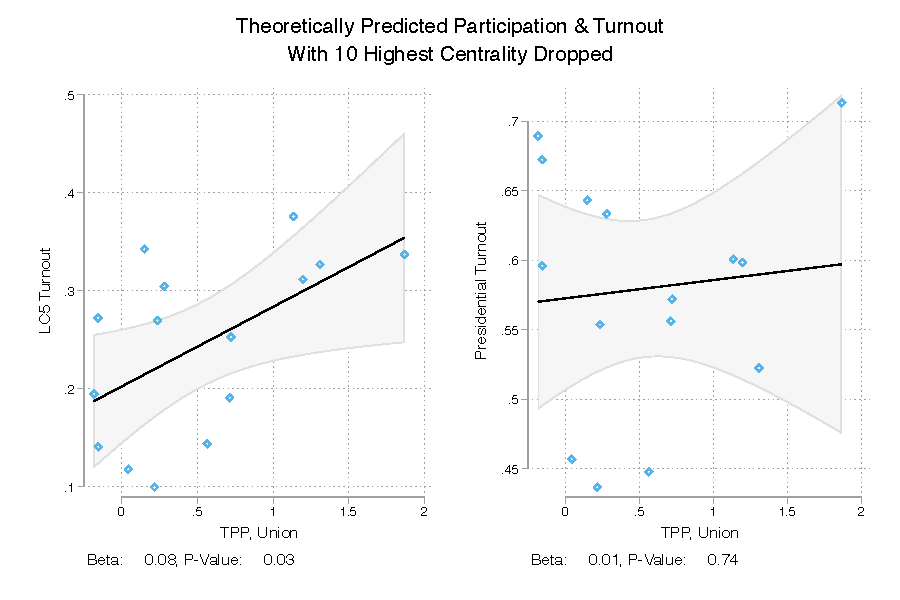
\includegraphics[width=0.7\textwidth]{../3_results/context_voting_scatter_drop10.pdf}
  \end{center}
	\scriptsize{\emph{Notes:}  The above plot presents the partial correlation between voter turnout in the Ugandan Presidential and LC5 Chair Elections and a modified version of TPP.  Grey bands indicate 95\% confidence intervals. In particular, TPP has been re-calculated by removing the ten individuals with highest eigenvector centrality from each network and re-running TPP simulations on those networks.}
\end{figure}

\begin{figure}[hb!]
  \begin{center}
    \caption{}\label{figure_context_voting_scatter_drop15}
      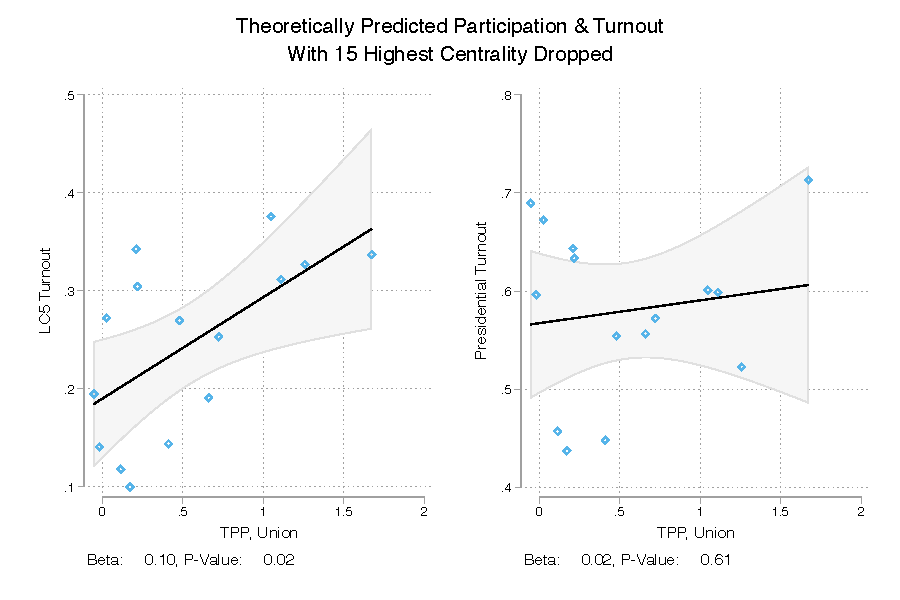
\includegraphics[width=0.7\textwidth]{../3_results/context_voting_scatter_drop15.pdf}
  \end{center}
	\scriptsize{\emph{Notes:}  The above plot presents the partial correlation between voter turnout in the Ugandan Presidential and LC5 Chair Elections and a modified version of TPP.  Grey bands indicate 95\% confidence intervals. In particular, TPP has been re-calculated by removing the fifteen individuals with highest eigenvector centrality from each network and re-running TPP simulations on those networks.}
\end{figure}

\pagebreak
\section{Information Diffusion Simulation}\label{appendix_diffusion_model}
We measure the ability of a network to efficiently diffuse information by running a simple diffusion model on our on empirical village networks. We then examine the average speed with which information spreads for each village.

Our decision to simulate this process is due to the fact that --- as with social context influences --- this is no simple statistic (like average degree or average shortest path length) which reliably summarizes the ability of a network to efficiently diffuse information when information spread is at least partially stochastic \citep[p. 19-35]{Newman:jyb}.

Our simulation proceeds as follows:
\begin{enumerate}
	\item At $t=0$, one vertex $v_0$ in the network (selected with uniform probability) is endowed with a unique piece of knowledge. It is thus ``informed'' ($I(v_0) = 1$). All other vertices are assumed to be ignorant of this knowledge ($I(v_j) = 0 \,\,\, \forall j\in V\backslash 0$).
	\item At $t=1$, information spreads from $v_0$ to each of the neighbors of $v_0$, denoted $N(v_0)$ with i.i.d. probability $\frac{p}{|N(v_0)|} \in(0,1)$.
	\item Step 2 is then repeated indefinitely, where at each stage all ``informed'' vertices spread their knowledge to neighbors with i.i.d. probability $p$.
\end{enumerate}

The ability of the network to support diffusion can then be specified as the number of people in the network that have become ``informed'' after $s$ steps of the diffusion model. The larger the number of people ``informed'' for a given number of steps $s$, the more efficient a village's network.

Note that the probability of information diffusion from a vertex to her neighbors is normalized by the number of neighbors. This can be thought of as approximating the idea that individuals can only have so many interactions in a given period of time. This normalization more closely approximates the idea that all individuals have the same probability of interacting and sharing information with at least \emph{a} friend in a given period, a dynamic suggested by recent work on information diffusion elsewhere in Uganda \citep{Larson:2016uz}. With that said, results look similar without the normalization.



\subsection{Information Diffusion Summary Statistics}
Table~\ref{diffusion_corr} below shows the correlation in the share of individuals in each village informed at different step thresholds, with different spread probabilities, and with different network specifications. As the table shows, inter-parameter correlations are quite high, and so an index is created for expositional ease by taking the first component of a PCA index for each network specification.

\begin{landscape}
    \begin{table}[htbp]\centering \caption{Diffusion Correlations across Parameter Values\label{diffusion_corr}}
\begin{tabular}{l  c  c  c  c }\hline\hline
\multicolumn{1}{c}{Variables} &p 0.60, 10 steps, Union&p 0.60, 20 steps, Union&p 0.35, 10 steps, Union&p 0.35, 20 steps, Union\\ \hline
p 0.60, 10 steps, Union&1.00\\
p 0.60, 20 steps, Union&0.76&1.00\\
p 0.35, 10 steps, Union&0.96&0.60&1.00\\
p 0.35, 20 steps, Union&0.97&0.83&0.92&1.00\\
\hline \hline 
 \end{tabular}
\end{table}

\end{landscape}

\section{Information Measures, Turnout, and TPP Regressions}\label{appendix_inforegs}


\begin{table}
\centering
\caption{Turnout and TPP with Information Measure Controls}\label{}
{
\def\sym#1{\ifmmode^{#1}\else\(^{#1}\)\fi}
\begin{tabular}{l*{4}{c}}
\toprule
                &\multicolumn{1}{c}{(1)}&\multicolumn{1}{c}{(2)}&\multicolumn{1}{c}{(3)}&\multicolumn{1}{c}{(4)}\\
                &\multicolumn{1}{c}{LC5 Chair}&\multicolumn{1}{c}{LC5 Chair}&\multicolumn{1}{c}{Presidential}&\multicolumn{1}{c}{Presidential}\\
\midrule
Eqm Participation Index (Union)&    0.055\sym{**} &    0.044\sym{*}  &    0.016         &   0.0053         \\
                &  (0.019)         &  (0.022)         &  (0.021)         &  (0.025)         \\
Share of Village Aware of UBridge&     0.33\sym{*}  &                  &     0.37\sym{*}  &                  \\
                &   (0.16)         &                  &   (0.18)         &                  \\
Info Diffusion Simulation 1st Component&                  &  -0.0020         &                  &   0.0011         \\
                &                  &  (0.012)         &                  &  (0.014)         \\
\midrule
Observations    &       15         &       15         &       15         &       15         \\
\bottomrule
\multicolumn{5}{l}{\footnotesize Standard errors in parentheses}\\
\multicolumn{5}{l}{\footnotesize \sym{*} \(p<0.1\), \sym{**} \(p<0.05\), \sym{***} \(p<0.01\)}\\
\end{tabular}
}

\end{table}

\clearpage
\pagebreak

\section{Village Network Plots}
\begin{figure}[bh!]
  \centering
  \caption{\protect237 Vertices, 1,457 Edges. Eqm Participation Index Value: -1.25}
  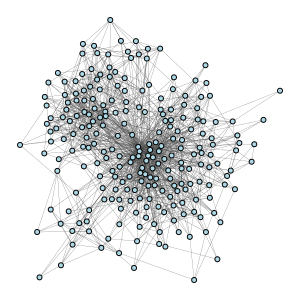
\includegraphics[width=0.7\textwidth]{../3_results/town_0.png} \\
\end{figure}
\begin{figure}
  \centering
  \caption{\protect229 Vertices, 1,723 Edges. Eqm Participation Index Value: 0.38}
  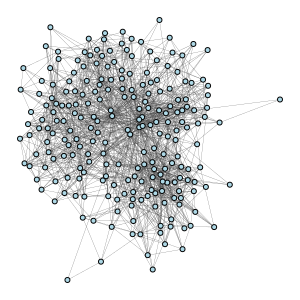
\includegraphics[width=0.7\textwidth]{../3_results/town_1.png} \\
\end{figure}
\begin{figure}
  \centering
  \caption{\protect204 Vertices, 1,618 Edges. Eqm Participation Index Value: 0.28}
  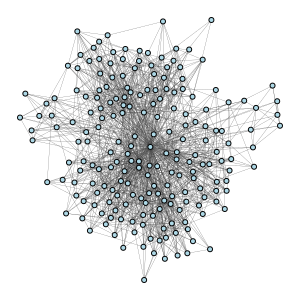
\includegraphics[width=0.7\textwidth]{../3_results/town_2.png} \\
\end{figure}
\begin{figure}
  \centering
  \caption{\protect197 Vertices, 1,283 Edges. Eqm Participation Index Value: -0.69}
  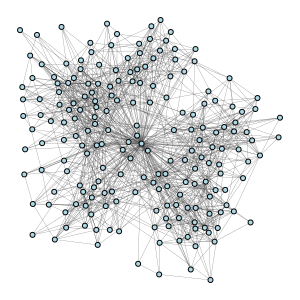
\includegraphics[width=0.7\textwidth]{../3_results/town_3.png} \\
\end{figure}
\begin{figure}
  \centering
  \caption{\protect30 Vertices, 176 Edges. Eqm Participation Index Value: -6.93}
  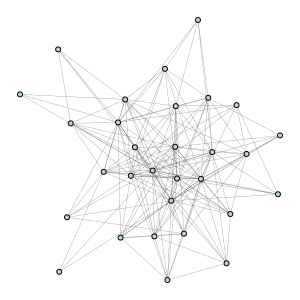
\includegraphics[width=0.7\textwidth]{../3_results/town_4.png} \\
\end{figure}
\begin{figure}
  \centering
  \caption{\protect189 Vertices, 1,370 Edges. Eqm Participation Index Value: -0.00}
  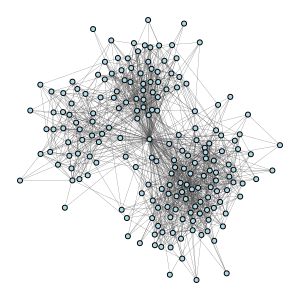
\includegraphics[width=0.7\textwidth]{../3_results/town_5.png} \\
\end{figure}
\begin{figure}
  \centering
  \caption{\protect283 Vertices, 2,797 Edges. Eqm Participation Index Value: 2.47}
  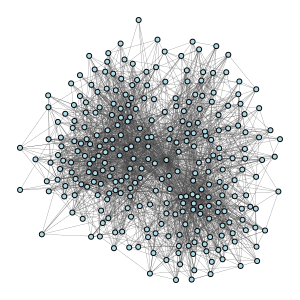
\includegraphics[width=0.7\textwidth]{../3_results/town_6.png} \\
\end{figure}
\begin{figure}
  \centering
  \caption{\protect192 Vertices, 1,490 Edges. Eqm Participation Index Value: 0.45}
  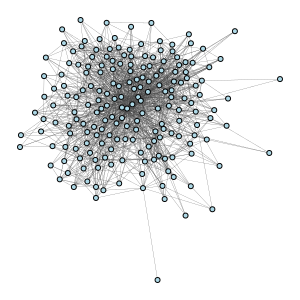
\includegraphics[width=0.7\textwidth]{../3_results/town_7.png} \\
\end{figure}
\begin{figure}
  \centering
  \caption{\protect163 Vertices, 1,247 Edges. Eqm Participation Index Value: -0.10}
  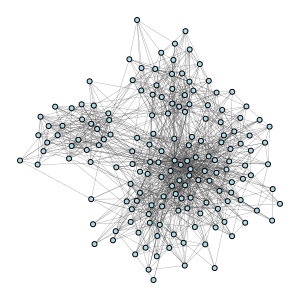
\includegraphics[width=0.7\textwidth]{../3_results/town_8.png} \\
\end{figure}
\begin{figure}
  \centering
  \caption{\protect168 Vertices, 1,189 Edges. Eqm Participation Index Value: -0.58}
  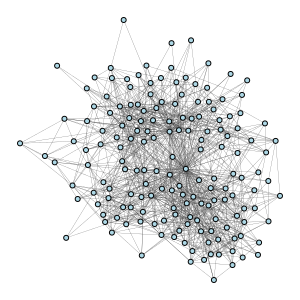
\includegraphics[width=0.7\textwidth]{../3_results/town_9.png} \\
\end{figure}
\begin{figure}
  \centering
  \caption{\protect254 Vertices, 2,423 Edges. Eqm Participation Index Value: 1.73}
  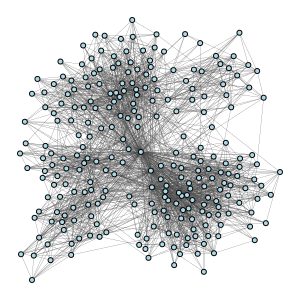
\includegraphics[width=0.7\textwidth]{../3_results/town_10.png} \\
\end{figure}
\begin{figure}
  \centering
  \caption{\protect225 Vertices, 2,016 Edges. Eqm Participation Index Value: 1.22}
  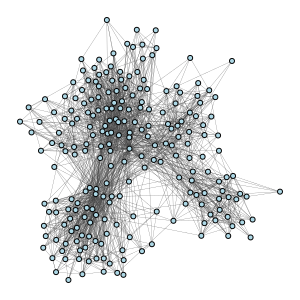
\includegraphics[width=0.7\textwidth]{../3_results/town_11.png} \\
\end{figure}
\begin{figure}
  \centering
  \caption{\protect205 Vertices, 1,857 Edges. Eqm Participation Index Value: 1.48}
  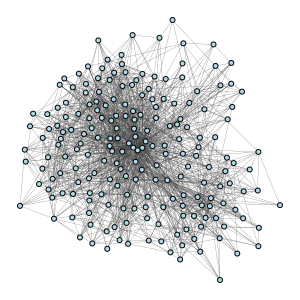
\includegraphics[width=0.7\textwidth]{../3_results/town_12.png} \\
\end{figure}
\begin{figure}
  \centering
  \caption{\protect263 Vertices, 2,272 Edges. Eqm Participation Index Value: 1.44}
  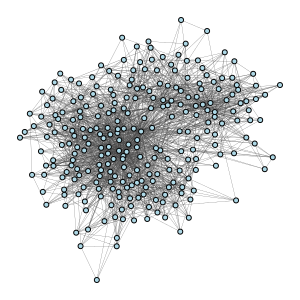
\includegraphics[width=0.7\textwidth]{../3_results/town_13.png} \\
\end{figure}
\begin{figure}
  \centering
  \caption{\protect185 Vertices, 1,516 Edges. Eqm Participation Index Value: 0.54}
  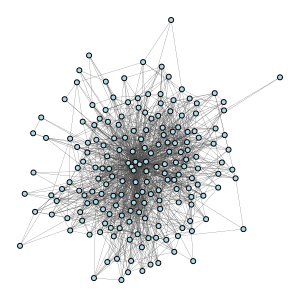
\includegraphics[width=0.7\textwidth]{../3_results/town_14.png} \\
\end{figure}
\begin{figure}
  \centering
  \caption{\protect160 Vertices, 1,150 Edges. Eqm Participation Index Value: -0.45}
  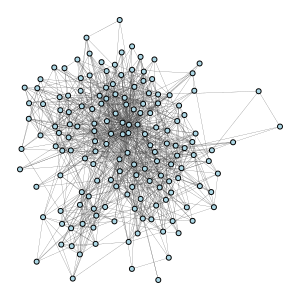
\includegraphics[width=0.7\textwidth]{../3_results/town_15.png} \\
\end{figure}


\end{appendix}

\end{document}
